\chapter{Algoritmi deterministici}



% TODO: Estendere a MaxMatching?
\section{\BiMaxMatching}
Sia $G=(V,E)$ un grafo non orientato. Un \emph{matching} (matrimonio) in $G$ è una selezione di lati in $E$ tale che su nessun vertice in $V$ incide più di un lato.
\MaxMatching è il problema di trovare il matching di cardinalità massima in un dato grafo.

\BiMaxMatching è una versione di \MaxMatching su grafi bipartiti, cioè in cui i vertici sono divisi in due classi e ogni lato incide su un vertice per classe: $G=(V_1,V_2,E)$ dove $V_1\cup V_2=\emptyset$ e $E\subseteq V_1\times V_2$. $\BiMaxMatching\in\PO$.

\popt{\BiMaxMatching}
{Grafo bipartito $G=(V_1,V_2,E)$}
{$X\subseteq E$}
{Determinare il matching di cardinalità massima in $G$}
{$X\subseteq E$}
{$\MAX$}
{$\card X$}

\begin{figure}
	\centering
	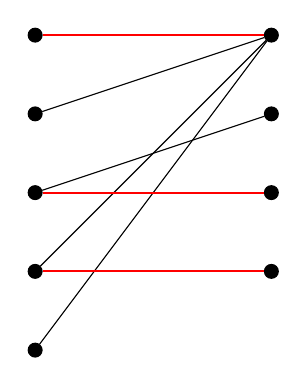
\begin{tikzpicture}[every node/.style={draw,inner sep=0pt,minimum size=5pt,fill,circle},matching/.style={red,thick}]
	\node at (0,1) (a) {};
	\node at (0,2) (b) {};
	\node at (0,3) (c) {};
	\node at (0,4) (d) {};
	\node at (0,5) (e) {};

	\node at (3,2) (f) {};
	\node at (3,3) (g) {};
	\node at (3,4) (h) {};
	\node at (3,5) (i) {};

	\draw		(a) -- (i);
	\draw		(b) -- (i);
	\draw		(d) -- (i);
	\draw[matching]	(e) -- (i);
	\draw[matching]	(b) -- (f);
	\draw[matching]	(c) -- (g);
	\draw		(c) -- (h);
\end{tikzpicture}

	\caption{Esempio di grafo bipartito. I lati colorati rappresentano un possibile matching.}
	\label{fig:graphmatching}
\end{figure}

Fissato un matching $M\subseteq E$, un lato $l\in E$ si dice \emph{occupato} se $l\in M$ e \emph{libero} se $l\notin M$.
Un vertice si dice \emph{esposto} se e solo se su di esso incidono solo lati liberi. Un cammino semplice si dice \emph{aumentante} rispetto a un matching se alterna lati liberi e occupati e inizia e termina su vertici esposti.
Quando un matching ha un cammino aumentante si può fare un \flang{flip}, cioè invertire l'appartenenza al matching dei lati del cammino aumentante.

\begin{figure}
	\centering
	\begin{subfigure}[b]{0.4\textwidth}
		\centering
		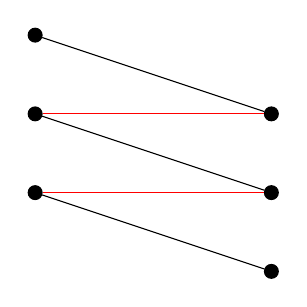
\begin{tikzpicture}
	\node[draw,inner sep=0pt,minimum size=5pt,fill, circle] at (3, 1)  (a) {};
	\node[draw,inner sep=0pt,minimum size=5pt,fill, circle] at (0, 2)  (b) {};
	\node[draw,inner sep=0pt,minimum size=5pt,fill, circle] at (0, 3)  (c) {};
	\node[draw,inner sep=0pt,minimum size=5pt,fill, circle] at (3, 2)  (f) {};
	\node[draw,inner sep=0pt,minimum size=5pt,fill, circle] at (3, 3)  (g) {};
	\node[draw,inner sep=0pt,minimum size=5pt,fill, circle] at (0, 4)  (h) {};

	\draw (a) -- (b);
	\draw[red] (b) -- (f);
	\draw (f) -- (c);
	\draw[red] (c) -- (g);
	\draw (g) -- (h);
\end{tikzpicture}

		\subcaption{Prima del flip.}
	\end{subfigure}
	\begin{subfigure}[b]{0.4\textwidth}
		\centering
		\input{img/matching_aumentante_post.tikz}
		\subcaption{Dopo il flip.}
	\end{subfigure}
	\caption{Esempio di cammino aumentante in un grafo bipartito.}
	\label{fig:augpaths}
\end{figure}

Vale il seguente teorema relativo ai cammini aumentanti per matching su grafi:
\begin{theorem}
	Sia $M$ un matching per un grafo $G$. Allora:
	\begin{equation*}
		\text{Esiste un cammino aumentante per $M$} \iff \text{$M$ non è massimo per $G$.}
	\end{equation*}
\end{theorem}
\begin{proof}~
	\begin{description}
		\item[$\Rightarrow$)] Applicando un flip al cammino aumentante si aumenta il matching di $1$.
		\item[$\Leftarrow$)] Se $M$ non è massimo, sia $M'$ il matching massimo per $G$ e sia $X:=(M\setminus M')\cup(M'\setminus M)$ (la differenza simmetrica di $M$ e $M'$).
			Su ogni vertice di $G$ possono incidere al più $2$ lati di $X$ (uno per ciascuno dei due matching).
			Nel grafo indotto da $X$, in ogni circuito l'appartenenza dei lati a $M$ e $M'$ è alternata e quindi il circuito è composto dallo stesso numero di lati di $M$ e di $M'$.
			Siccome però $M'$ ha più lati di $M$, esiste almeno un cammino semplice nel grafo indotto da $X$ che ha più lati in $M'$.
			Tale cammino alterna lati di $M$ e di $M'$ ed è aumentante rispetto a $M$ in $G$.
	\end{description}
\end{proof}

% TODO: è necessario discutere di come viene effettuata la visita per FindAugmenting e quale sia la sua complessità. Tenere conto di ciò nel paragone con MaxMatching: è possibile usare lo stesso algoritmo su grafi non bipartiti?
\SetKwFunction{FindAugmenting}{FindAugmenting}
\SetKwFunction{Flip}{Flip}
L'algoritmo \ref{alg:BiMaxMatching} risolve \BiMaxMatching trovando l'ottimo in tempo polinomiale.
La procedura \FindAugmenting tiene traccia dei vertici esposti e fa una visita in profondità del grafo a partire da uno di essi, alternando lati liberi e occupati, identificando un cammino aumentante.
La procedura \Flip esegue un flip del matching dato.

\begin{algorithm}
	$M \asn \emptyset$\;
\While{}{
	$\pi\asn\FindAugmenting{G,M}$\;
	\If{$\pi=\bot$}{
		\Return $M$\;
	}\Else{
		$M\asn\Flip(M,\pi)$\;
	}
}

	\caption{Risoluzione polinomiale di \BiMaxMatching}
	\label{alg:BiMaxMatching}
\end{algorithm}

\begin{corollario}
	$\BiMaxMatching\in\PO$.
\end{corollario}

\PerfectMatching è il problema di decisione che si chiede se in un grafo bipartito esista un matching che coinvolge tutti i vertici.

\begin{corollario}
	$\PerfectMatching\in\P$.
\end{corollario}



\section{\LoadBalancing}
Il problema \LoadBalancing (bilanciamento del carico) consiste nel dividere un insieme di task, ciascuno con la sua durata, tra le macchine di un insieme, in modo da minimizzare la durata complessiva (carico) impiegata dalla macchina più lenta. Questo problema è \NPO-completo.

\popt
{\LoadBalancing}
{Durate $t_0,\dots,t_{n-1}\in\N^+$ per $n$ task, numero $m$ di macchine}
{Assegnamento di ciascun task a una macchina}
{Determinare l'assegnamento che minimizza la durata massima}
{Assegnamenti $x:n\to m$}
{$\MIN$}
{$L=\max_j L_j$, dove $L_j:=\sum_{i\in x^{-1}(j)} t_i$}


\subsection{\GreedyLoadBalancing}
Un algoritmo greedy può trovare una soluzione ammissibile per \LoadBalancing.
L'algoritmo esamina i task $t_0,t_1,\dots,t_{n-1}$ nell'ordine, assegnando ogni task alla macchina più scarica.
\GreedyLoadBalancing, se implementato con una coda con priorità che tenga conto della macchina dal carico minimo (effettuando $n$ operazioni di insert/update per i carichi di $m$ macchine), opera in tempo $O(n\log m)$.
L'algoritmo non ottiene, in generale, la soluzione ottima, ma ha la garanzia di non produrre più del doppio dell'ottimo, come dimostrato dal seguente teorema:

\begin{theorem}\label{thm:greedyloadbalancing}
	\GreedyLoadBalancing è un algoritmo 2-approssimante per \LoadBalancing.
\end{theorem}
Prima di dimostrare il teorema si consideri il seguente lemma:
\begin{lemma}\label{lem:load:ultimopasso}
	Sia $L\star$ il costo della soluzione ottima. Sia $\bar j$ tale che $L_{\bar j}=L\star$ e sia $\bar i$ l'ultimo task assegnato a $\bar j$. Allora:
	\begin{equation*}
		L_{\bar j}-t_{\bar i} \leq L\star
	\end{equation*}
\end{lemma}
\begin{proof}
	Il carico della macchina $\bar j$ prima dell'assegnamento $\bar i$ era $L_{\bar j}-t_{\bar i}$, il cui era minore di ogni altro carico per via di come l'algoritmo sceglie a chi assegnare.
	Indicato con $L\star_j$ il carico della macchina $j$ nella soluzione ottima, vale $L\star\geq\frac1m\sum_it_i$, essendo $mL\star\geq\sum_jL\star_j=\sum_it_i$.
	\begin{gather*}
		L_{\bar j}-t_{\bar i}\leq L_j \qquad\forall j \\
		\sum_j (L_{\bar j}-t_{\bar i})\leq\sum_j L_j=\sum_i t_i\\
		m(L_{\bar j}-t_{\bar i})\leq \sum_i t_i \\
		L_{\bar j}-t_{\bar i}\leq\frac1m\sum_j t_j\leq L\star
	\end{gather*}
\end{proof}
Si può ora procedere con la dimostrazione del teorema \ref{thm:greedyloadbalancing}:
\begin{proof}
	Si osservi che $L\star\geq\max_it_i$. Applicando il lemma \ref{lem:load:ultimopasso}:
	\begin{gather*}
		L=L_{\bar j}=\underbrace{L_{\bar j}-t_{\bar i}}_{\leq L\star}+\underbrace{t_{\bar i}}_{\leq L\star}\leq 2L\star \\[1ex]
		\frac L{L\star}\leq 2
	\end{gather*}
\end{proof}

\begin{corollario}
	$\LoadBalancing\in\gAPX2$.
\end{corollario}

Si dimostra che questo risultato sull'analisi di \GreedyLoadBalancing è tight:
\begin{theorem}
	Per ogni $\varepsilon>0$ esiste un input di \LoadBalancing su cui \GreedyLoadBalancing produce una soluzione $L$ tale che
	\begin{equation*}
		2-\varepsilon\leq\frac L{L\star}\leq2
	\end{equation*}
\end{theorem}
\begin{proof}
	Scegliamo un numero di macchine $m>\frac1\varepsilon$ e un numero di task $n=m(m-1)+1$. Questi task consistono, nell'ordine, in $n-1$ task da $1$ e un task da $m$. Naturalmente la soluzione ottima assegna unicamente il task da $m$ a una macchina, che risulta la più carica, quindi $L\star=m$.

	Per assegnare i task, l'algoritmo assegna un task da $1$ per ogni macchina ciclicamente finché arriva il task da $m$, che viene assegnato a una macchina di carico $m-1$ producendo un costo finale di $2m-1$. In questo caso si ha
	\begin{equation*}
		\frac L{L\star}=\frac{2m-1}{m}=2-\frac1m\geq2-\varepsilon
	\end{equation*}
\end{proof}


\subsection{\SortedGreedyBalance}
Un algoritmo \SortedGreedyBalance può ordinare i task in ordine decrescente prima di assegnarli come \GreedyLoadBalancing. Questo algoritmo ha costo in tempo di $O(n\log n+n\log m)$.

\begin{theorem}
	\SortedGreedyBalance è un algoritmo $\frac32$-approssimante per \LoadBalancing.
\end{theorem}
\begin{proof}
	Se $n\leq m$ la soluzione è ottima e la tesi è ovvia.

	Se $n>m$, esiste una macchina che riceve due task. Il primo task assegnato a una macchina già carica è $t_m$, e vale:
	\begin{equation*}
		L\star\geq 2t_m
	\end{equation*}

	Sia $\bar j$ la macchina con carico massimo al termine dell'esecuzione e $\bar i$ l'ultimo carico assegnato. Si ha $\bar i \geq m$, da cui $t_{\bar i}\leq t_m$ e quindi $t_{\bar i}\leq t_m\leq \frac12 L\star$.
	\begin{gather*}
		L=\underbrace{L_{\bar j}-t_{\bar i}}_{\leq L\star}+\underbrace{t_{\bar i} }_{\leq \frac12 L\star}\leq L\star+\frac12 L\star=\frac32L\star
	\end{gather*}
\end{proof}

Valgono inoltre i seguenti teoremi riguardanti \LoadBalancing, che non dimostriamo.
\begin{theorem}~
	\begin{itemize}
		% TODO: add bib
		\item \SortedGreedyBalance è un algoritmo $\frac43$-approssimante per \LoadBalancing \cite{Graham:69:sortedgreedybalance};
		\item $\LoadBalancing\in\PTAS$;
		\item $\P\neq\NP\impl\LoadBalancing\notin\FPTAS$.
	\end{itemize}
\end{theorem}



\section{\CenterSelection}
Nel problema \CenterSelection è dato uno spazio metrico $\tuple{S,d}$ di punti.
Si vuole minimizzare la distanza massima $\rho(C)$ tra un nodo e il suo nodo di riferimento, detta raggio di copertura.
\CenterSelection è un problema \NPO-completo.

\popt{\CenterSelection}
{Insieme $S$ di punti, metrica $d$, numero massimo di centri $k\in\N^+$}
{Centri $C\subseteq S$}
{Quali centri selezionare in modo da minimizzare il raggio di copertura}
{$C\subseteq S\mid \card C\leq k$}
{$\MIN$}
{$\rho(C) = \max_{x \in S} d(x, C)$}

Uno spazio metrico è un insieme $\Omega$ di punti su cui vale una funzione distanza $d:\Omega\times\Omega\to\R^{\geq0}$ tale che:
\begin{itemize}
	\item $d(x,y)=0\iff x=y$
	\item $d(x,y)=d(y,x)\forall x,y\in\Omega$
	\item $d(x,y)=d(x,z)+d(z,y)$ (disuguaglianza triangolare)
\end{itemize}

\begin{defin}[tassellificazione di Voronoi]
	Dato uno spazio metrico $\tuple{\Omega,d}$, sia $S\subseteq\Omega$ finito e $C\subseteq S$ l'insieme dei centri. Per ogni $c\in C$ la cella di Voronoi rispetto al centro $c$ è l'insieme dei punti $s\in S$ tali che
	\begin{equation*}
		c=\arg\min_{c'\in C} d(s,c')
	\end{equation*}
	% TODO: brutta, esprimere meglio
	Dato un punto $s\in S$ definiamo l'assegnamento di $s$ alla cella di centro $c\in C$ $\text{VC}_C(s)=\arg\min_{c'\in C} d(s,c')$.
\end{defin}

\begin{equation*}
	\text{VC}_C(s)=\arg\min_{c\in C} d(s,c)
\end{equation*}

\CenterSelection è il problema che riceve in input $S\subseteq_\text{fin}\Omega$ e $k\in\N^+$, ha come soluzioni ammissibili le selezioni di centri $C\subseteq S$ con $\card C\leq k$ e come obiettivo da minimizzare:
\begin{equation*}
	\rho(C)=\max_{s\in S} d(s,\text{VC}_C(s))
\end{equation*}

\subsection{\CenterSelectionPlus}
L'algoritmo \ref{alg:CenterSelectionPlus} non risolve \CenterSelection in quanto richiede un input $r$ aggiuntivo rispetto a quelli previsti dal problema, che consiste in una stima del raggio di copertura ottimo $r\star$.

\begin{algorithm}[ht]
	\caption{\CenterSelectionPlus}
	\label{alg:CenterSelectionPlus}
	\SetKwFunction{ExtractRandomPoint}{ExtractRandomPoint}

\KwInput{$S$, $k$, $d$, $r$}

$C\asn\emptyset$\;
\While{$S \neq \emptyset$}{
	$\bar s\asn\ExtractRandomPoint(S)$\;
	$C\asn C\cup \set{\bar s}$\;
	$S\asn S\setminus\set{x\mid d(x,\bar s)\leq 2r}$\;
}
\If{$\card C\leq k$}{
	\Return $C$\;
}\Else{
	Impossibile\;
}

\end{algorithm}

Si noti che un algoritmo \CenterSelectionPlus' che, invece di eliminare punti di $S$, non prenda in considerazione nella selezione di nuovi centri punti $s$ tali che $d(s,C)>2r$, è del tutto equivalente a \CenterSelectionPlus.
\begin{theorem}
	Valgono le seguenti proprietà per \CenterSelectionPlus:
	\begin{enumerate}[(a)]
		\item \label{itm:centerselection:plus1} se l'algoritmo emette un output $C$, allora $C$ è una soluzione ammissibile con $\rho(C)\leq 2r$;
		\item \label{itm:centerselection:plus2} se $r\geq\rho\star$ allora l'algoritmo emette un output.
	\end{enumerate}
\end{theorem}
\begin{proof}
	\ref{itm:centerselection:plus1} L'output $C$ è ammissibile in quanto composto da elementi di $S$ e $\card C\leq k$. Poiché l'algoritmo termina quando sono stati eliminati tutti i punti di $S$, e ogni punto $\bar s\in S$ viene eliminato quando per un centro $\bar s$ selezionato vale $d(s,\bar s\leq 2r$, il raggio massimo da un punto al centro più vicino è minore o uguale a $2r$;

	\ref{itm:centerselection:plus2} Sia $C\star$ una soluzione ottima. Si consideri $\bar s\in S$ e sia $\bar c:=\text{VC}_{C\star}(\bar s)$ e $X_{\bar c}:=\text{VC}_{C\star}^{-1}(\bar c)$.
	Per qualunque punto $s\in X_{\bar c}$ vale, per disuguaglianza triangolare:
	\begin{align*}
		d(s,\bar s) & \leq d(s,c\star(s))+d(c\star(s),\bar s)                \\
		            & = d(s,c\star(s))+d(c\star(\bar s),\bar s)              \\
		            & \leq \rho\star + \rho\star = 2\rho\star \leq 2r \text.
	\end{align*}
	Quindi dopo l'inserimento di $\bar s$ non rimane in $S$ alcun elemento di $X_{\bar c)}$. Poiché la soluzione ottima contiene al più $k$ centri, dopo al più $k$ iterazioni tutti i punti di $S$ sono stati rimossi, e $\card C\leq k$.
\end{proof}


Come rappresentato in figura \ref{fig:csplus_r_beh}, l'algoritmo ricevendo $r\geq\rho\star$ produce una soluzione ammissibile con approssimazione $\frac{2r}{\rho\star}$; se $r\leq\frac{\rho\star}{2}$ l'algoritmo non produce output; nei casi rimanenti il comportamento dell'algoritmo non è consistente.
Un algoritmo del genere può essere utilizzato sfruttando un'opportuna applicazione della ricerca dicotomica per la determinazione del valore ottimo di $r$.

\begin{figure}[ht]
	\centering
	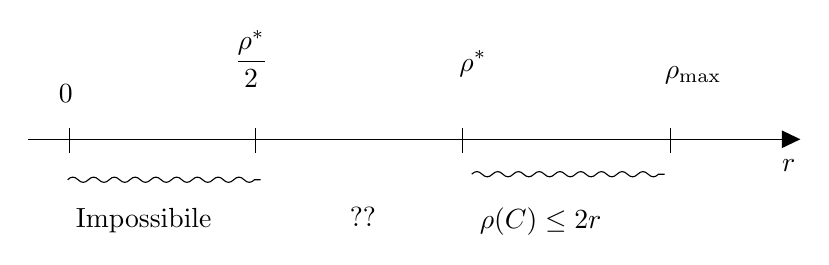
\begin{tikzpicture}[x=0.75pt,y=0.75pt,yscale=-1,xscale=1]
	\draw    (121,120.5) -- (490,120.5) ;
	\draw [shift={(493,120.5)}, rotate = 180] [fill={rgb, 255:red, 0; green, 0; blue, 0 }  ][line width=0.08]  [draw opacity=0] (8.93,-4.29) -- (0,0) -- (8.93,4.29) -- cycle    ;
	\draw    (230.33,115) -- (230.33,127) ;
	\draw    (330.33,115) -- (330.33,127) ;
	\draw    (430.33,115) -- (430.33,127) ;
	\draw    (140.75,115) -- (140.75,127) ;
	\draw    (140,140) .. controls (141.67,138.33) and (143.33,138.33) .. (145,140) .. controls (146.67,141.67) and (148.33,141.67) .. (150,140) .. controls (151.67,138.33) and (153.33,138.33) .. (155,140) .. controls (156.67,141.67) and (158.33,141.67) .. (160,140) .. controls (161.67,138.33) and (163.33,138.33) .. (165,140) .. controls (166.67,141.67) and (168.33,141.67) .. (170,140) .. controls (171.67,138.33) and (173.33,138.33) .. (175,140) .. controls (176.67,141.67) and (178.33,141.67) .. (180,140) .. controls (181.67,138.33) and (183.33,138.33) .. (185,140) .. controls (186.67,141.67) and (188.33,141.67) .. (190,140) .. controls (191.67,138.33) and (193.33,138.33) .. (195,140) .. controls (196.67,141.67) and (198.33,141.67) .. (200,140) .. controls (201.67,138.33) and (203.33,138.33) .. (205,140) .. controls (206.67,141.67) and (208.33,141.67) .. (210,140) .. controls (211.67,138.33) and (213.33,138.33) .. (215,140) .. controls (216.67,141.67) and (218.33,141.67) .. (220,140) .. controls (221.67,138.33) and (223.33,138.33) .. (225,140) .. controls (226.67,141.67) and (228.33,141.67) .. (230,140) -- (233,140) -- (233,140) ;
	\draw    (334.67,137.33) .. controls (336.34,135.66) and (338,135.66) .. (339.67,137.33) .. controls (341.34,139) and (343,139) .. (344.67,137.33) .. controls (346.34,135.66) and (348,135.66) .. (349.67,137.33) .. controls (351.34,139) and (353,139) .. (354.67,137.33) .. controls (356.34,135.66) and (358,135.66) .. (359.67,137.33) .. controls (361.34,139) and (363,139) .. (364.67,137.33) .. controls (366.34,135.66) and (368,135.66) .. (369.67,137.33) .. controls (371.34,139) and (373,139) .. (374.67,137.33) .. controls (376.34,135.66) and (378,135.66) .. (379.67,137.33) .. controls (381.34,139) and (383,139) .. (384.67,137.33) .. controls (386.34,135.66) and (388,135.66) .. (389.67,137.33) .. controls (391.34,139) and (393,139) .. (394.67,137.33) .. controls (396.34,135.66) and (398,135.66) .. (399.67,137.33) .. controls (401.34,139) and (403,139) .. (404.67,137.33) .. controls (406.34,135.66) and (408,135.66) .. (409.67,137.33) .. controls (411.34,139) and (413,139) .. (414.67,137.33) .. controls (416.34,135.66) and (418,135.66) .. (419.67,137.33) .. controls (421.34,139) and (423,139) .. (424.67,137.33) -- (427.67,137.33) -- (427.67,137.33) ;

	\draw (483,129) node [anchor=north west][inner sep=0.75pt]   [align=left] {$\displaystyle r$};
	\draw (134.5,93) node [anchor=north west][inner sep=0.75pt]   [align=left] {$\displaystyle 0$};
	\draw (219,67) node [anchor=north west][inner sep=0.75pt]   [align=left] {$\displaystyle \frac{\rho ^{*}}{2}$};
	\draw (327.5,76.5) node [anchor=north west][inner sep=0.75pt]   [align=left] {$\displaystyle \rho ^{*}$};
	\draw (426.5,84) node [anchor=north west][inner sep=0.75pt]   [align=left] {$\displaystyle \rho_{\max}$};
	\draw (142.67,152.67) node [anchor=north west][inner sep=0.75pt]   [align=left] {Impossibile};
	\draw (337.33,152) node [anchor=north west][inner sep=0.75pt]   [align=left] {$\rho(C)\leq 2r$};
	\draw (274.67,152) node [anchor=north west][inner sep=0.75pt]   [align=left] {??};
\end{tikzpicture}

	\caption{Comportamento di \CenterSelectionPlus.}
	\label{fig:csplus_r_beh}
\end{figure}


\subsection{\GreedyCenterSelection}
L'algoritmo \ref{algo:GreedyCenterSelection} è un algoritmo greedy per \CenterSelection.

\begin{algorithm}
	\caption{\GreedyCenterSelection}
	\SetKwFunction{ExtractRandomPoint}{ExtractRandomPoint}

\KwInput{$S$, $k$, $d$}

\If{$\card S\leq k$}{
	\Return $S$\;
}
$s\asn\ExtractRandomPoint(S)$\;
$C\asn C\cup \set{s}$\;
\While{$\card C\leq k$}{
	$\bar s\asn\arg\max_{s\in S} d(s,C)$\;
	$C\asn C\cup\set{\bar s}$\;
}
\Return $C$\;

	\label{algo:GreedyCenterSelection}
\end{algorithm}

\begin{theorem}
	\GreedyCenterSelection è un algoritmo $2$-approssimante per \CenterSelection.
\end{theorem}
\begin{proof}
	Per assurdo, supponiamo che $C$ sia tale che $\rho(C)>2\rho\star$, ossi  esiste $\hat s\in S$ tale che $d(\hat s,C)> 2\rho\star$.
	Consideriamo l'$i$-esima iterazione dell'algoritmo: sia $C_i$ l'insieme dei centri all'inizio dell'$i$-esima iterazione e $\bar s_i$ il centro da inserire. Vale:
	\begin{equation*}
		d(\bar s_i,C_i)\geq d(\hat s,C_i)\geq d(\hat s, C)>2\rho\star
	\end{equation*}
	Questa condizione è esattamente quella che esclude punti dalla selezione di \CenterSelectionPlus', pertanto i due algoritmi sono equivalenti se $r=\rho\star$. Ma per $r=\rho\star$ \CenterSelectionPlus' emette una $\frac{2\rho\star}{\rho\star}=2$-approssimazione, il che contraddice l'ipotesi di assurdo.
\end{proof}

\begin{theorem}
	Se $\P\neq\NP$, non esiste $\alpha<2$ tale che $\CenterSelection\in\gAPX\alpha$.
\end{theorem}
\begin{proof}
	Si consideri il problema di decisione \NP-completo \DominatingSet. Dato un grafo non orientato $G=(V,E)$, un dominating set per $G$ è un insieme di vertici $D\subseteq V$ se e solo se ogni vertice non appartenente a $D$ ha un adiacente in $D$: $\forall x\in(V\setminus D),\exists y\in D\mid \set{x,y}\in D$.

	\pdec{\DominatingSet}
	{Grafo non orientato $G=(V,E)$, $k\in\N^+$}
	{Determinare se esiste un dominating set per $G$ di cardinalità minore o uguale a $k$}

	Data un'istanza $((V,E),k)$ di \DominatingSet, costruiamo una istanza di \CenterSelection che ha per spazio l'insieme dei vertici, per numero massimo di centri il limite di cardinalità $k$ per il dominating set e per metrica la funzione
	\begin{equation*}
		d(x,y) =
		\begin{cases}
			0 \quad & \text{se } x = y                      \\
			1 \quad & \text{se } x\neq y\land\set{x,y}\in E \\
			2 \quad & \text{altrimenti}
		\end{cases}
	\end{equation*}

	In una istanza di \CenterSelection derivata in questo modo, $\rho\star=2$ oppure $\rho\star=1$. Nel secondo caso l'insieme di centri scelti è un dominating set nell'istanza originale del problema, infatti:
	\begin{align*}
		\rho\star=1 & \coimpl\forall x\in(V\setminus D)\quad d(x,D)=1                             \\
		            & \coimpl\forall x \in (V \setminus D)\quad \exists y\in D\mid d(x,y)=1       \\
		            & \coimpl\forall x \in (V \setminus D)\quad \exists y\in D\mid \set{x,y}\in E \\
		            & \coimpl D\text{ è un dominating set}
	\end{align*}

	Per assurdo, supponiamo che esista un algoritmo $\alpha$-approssimante per \CenterSelection, con $\alpha < 2$. Eseguendo tale algoritmo su un'istanza così costruita si ottiene un output $D$ tale che:
	\begin{gather*}
		1\leq\frac{\rho(D)}{\rho\star}\leq\alpha<2 \\
		\rho\star\leq\rho(D)\leq\alpha\cdot\rho\star<2\rho\star
	\end{gather*}

	Dato che $\rho\star=1\lor\rho\star=2$, allora vale esattamente una delle seguenti proposizioni:
	\begin{equation*}
		\begin{cases}
			1\leq\rho(D)<2\quad & \text{se } \rho\star=1 \\
			2\leq\rho(D)<4\quad & \text{se } \rho\star=2
		\end{cases}
	\end{equation*}
	Quindi, eseguito l'algoritmo, se $\rho(D)<2$ allora $\rho\star=1$ e la decisione per l'istanza originale di \DominatingSet è positiva; se $\rho(D)\geq2$ allora $\rho\star=2$ e la decisione è negativa.

	Poiché l'algoritmo agisce in tempo polinomiale, allora $\DominatingSet\in\P$, il che è assurdo se $\P\neq\NP$.
\end{proof}



\section{Problema della copertura d'insiemi}
Si definisce funzione armonica la funzione $H:\N^+\to\R$ tale che
\begin{equation*}
	H(n)=\sum_{k=1}^n \frac 1k
\end{equation*}

% TODO: dimostrare in un'appendice (vedi vecchi appunti)
Vale la seguente proprietà per la funzione armonica:
\begin{theorem}
	\begin{equation*}
		\ln(n+1)\leq H(n)\leq 1+\ln(n)
	\end{equation*}
\end{theorem}

\popt{\MinSetCover}
{$S_1,S_2,\dots,S_m\subseteq U$ tali che $\cup_{i=1}^m S_i=U$ e pesi $w_1,\dots,w_m$ con $w_i \in\R^{>0}~\forall i$}
{$C\subseteq\set{S_1,\dots,S_n}$}
{Quali sono gli insiemi da scegliere per coprire tutti gli elementi di $U$ col costo minore possibile?}
{$C$ tale che $\cup_{i\in C}S_i=U$}
{$\MIN$}
{$w:=\sum_{i:S_i\in C} w_i$}


\subsection{Algoritmo greedy set cover}
\begin{algorithm}[ht]
	\caption{\GreedySetCover}
	\label{algo:greedysetcover}
	\KwInput{$S_i, U$}

$R\asn U$\;
$C\asn\emptyset$\;
\While{$R\neq\emptyset$} {
	$i=\arg\min_i \set{\frac{w_i}{\card{S_i \cap R}}}$\;
	$C\asn C\cup\set{S_i}$\;
	$R\asn R\setminus S_i$\;
}
\Return{$C$}\;

\end{algorithm}
L'algoritmo \ref{algo:greedysetcover} costruisce polinomialmente una soluzione per \MinSetCover, scegliendo a ogni iterazione il sottoinsieme di input che minimizza il rapporto tra il suo peso e il numero di elementi che esso aggiunge all'output parziale.

Ogni elemento $s\in U$ viene inserito nell'output parziale in qualche iterazione $j$ con l'aggiunta di un sottoinsieme $S_j$. Definiamo quindi
\begin{equation*}
	c_u = \frac{w_j}{\card{S_j\cap R_j}}
\end{equation*}
il costo della copertura del singolo elemento di $U$, avvenuta tramite l'aggiunta di $S_j$ durante la $j$-esima iterazione.

\begin{lemma}\label{lem:gsetcov_w_sum_c_u}
	\begin{equation*}
		w=\sum_{u\in U} c_u
	\end{equation*}
\end{lemma}
\begin{proof}
	Si noti che gli insiemi $S_j\cap R_j$, dove $S_j$ è l'insieme di input scelto al passo $j$ e $R_j$ è l'insieme degli elementi dell'universo rimasti da selezionare al passo $j$, costituiscono una partizione di $U$. Infatti, l'algoritmo termina solo dopo aver esaurito gli elementi di $U$, e ogni insieme $S_j\cap R_j$ aggiunge unicamente nuovi elementi.

	Sia $w_j$ il costo dell'insieme $S_j$ aggiunto al passo $j$. Allora
	\begin{equation*}
		w = \sum_j w_j=\sum_j\sum_{s\in S_j\cap R_j} c_s=\sum_{u\in U} c_u
	\end{equation*}
\end{proof}
\begin{lemma}\label{lem:gsetcov_cu_leq_harmoskwk}
	\begin{equation*}
		\forall k\in\set{1,\dots,m} \quad\sum_{s\in S_k} c_u\leq H(\card{S_k}) \cdot w_k
	\end{equation*}
\end{lemma}
\begin{proof}
	Sia $S_k=\set{u_1,u_2,\dots,u_d}$, dove gli elementi sono elencati in ordine di copertura.

	Quando un elemento $s_j$ viene coperto dall'inserimento di un insieme $S_{k'}$, gli elementi di $S_k$ ancora da inserire spaziano almeno da $s_j$ a $s_d$, quindi:
	\begin{equation*}
		\card{S_k\cap R}\geq d-j+1 \text.
	\end{equation*}
	Quindi
	\begin{equation*}
		c_{s_j}=\frac{w_{k'}}{\card{S_{k'}\cap R_j}}
		\leq\frac{w_k}{\card{S_k\cap R_j}}
		\leq\frac{w_k}{d-j+1} \text.
	\end{equation*}
	E, di conseguenza
	\begin{align*}
		\sum_{s\in S_k} c_s & =c_{s_1}+c_{s_2}+c_{s_3}\dots+c_{s_d}                            \\
		                    & \leq \frac{w_k}{d-1+1}+\frac{w_k}{d-2+1}+\dots+\frac{w_k}{d-d+1} \\
		                    & \leq \frac{w_k}{d}+\frac{w_k}{d-1}+\dots+\frac{w_k}{1}           \\
		                    & = w_k\left(1 + \frac{1}{2} + \dots + \frac{1}{d}\right)          \\
		                    & = w_k\cdot H(\card{S_k})
	\end{align*}
\end{proof}

\begin{theorem}
	Sia $M=\max_i\card{S_i}$. \GreedySetCover è $H(M)$-approssimante per \MinSetCover.
\end{theorem}
\begin{proof}
	Sia $w\star:=\sum_{i:S_i\in C\star} w_i$.
	Applicato l'algoritmo, in virtù del lemma \ref{lem:gsetcov_cu_leq_harmoskwk} vale, per qualunque $i$:
	\begin{equation*}
		w_i\geq\frac{\sum_{s\in S_i} c_s}{H(\card{S_i})}\geq\frac{\sum_{s\in S_i} c_s}{H(M)}
	\end{equation*}
	Essendo $C\star$ una copertura e applicando il lemma \ref{lem:gsetcov_w_sum_c_u}:
	\begin{equation*}
		\sum_{S_i\in C\star}\sum_{s\in S_i} c_s \geq \sum_{s\in U} c_s = w
	\end{equation*}
	Applicando queste due osservazioni:
	\begin{gather*}
		w\star = \sum_{i:S_i\in C\star} w_i \geq \sum_{i:S_i\in C\star} \frac{\sum_{s\in S_i} c_s}{H(M)} \geq \frac{w}{H(M)} \\
		\frac{w}{w\star} \leq H(M)
	\end{gather*}
\end{proof}

Inoltre vale:
\begin{equation*}
	H(M)\leq H(\card U) = O(\ln(\card U))
\end{equation*}
Ergo:
\begin{corollario}
	\GreedySetCover è un algoritmo $O(\ln(n))$-approssimante per \MinSetCover, dove $n$ è la cardinalità dell'insieme universo.
\end{corollario}

Per quanto riguarda l'ottimalità di questo bound:
\begin{theorem}
	Per ogni $\varepsilon>0$, \GreedySetCover non è $(O(\ln(n))-\varepsilon)$-approssimante per \MinSetCover.
\end{theorem}
\begin{proof}
	% TODO: adattare a n non potenza di 2?
	Fissati $\varepsilon$ e $n$ (sia per semplicità $n=2^k$ per qualche $k\in\N^+,k>2$), si consideri l'input per \MinSetCover mostrato in figura \ref{fig:setcover_tightness}.
	L'input è costituito da due insiemi disgiunti $A$ e $B$ di costo $1+\varepsilon$ e cardinalità $n/2$; e $\log_2 n$ insiemi disgiunti $S_1,S_2,\dots,S_{\log_2 n}$, di cardinalità rispettive $n/2,n/4,\dots$ e costo $1$. In ciascun insieme $S_i$, metà degli elementi è contenuta in $A$ e l'altra metà in $B$.

	\begin{figure}[ht]
		\centering
		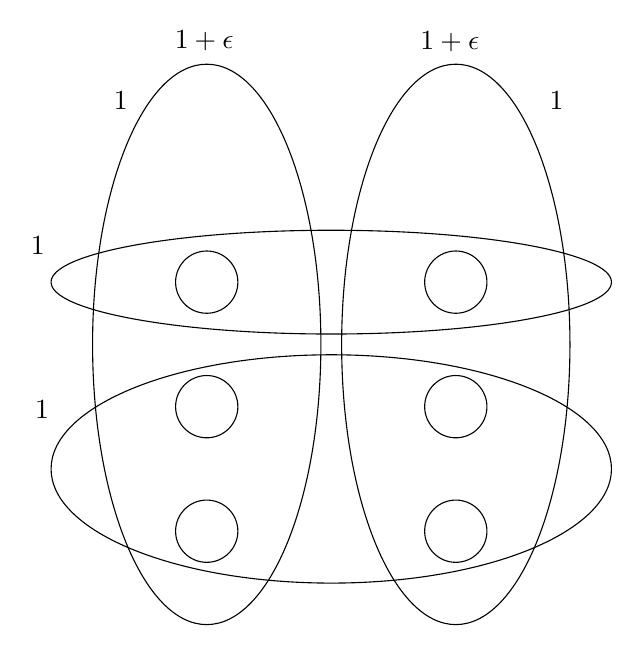
\begin{tikzpicture}[x=0.75pt,y=0.75pt,yscale=-1,xscale=1]
	\draw   (150,155) .. controls (150,80.44) and (174.62,20) .. (205,20) .. controls (235.38,20) and (260,80.44) .. (260,155) .. controls (260,229.56) and (235.38,290) .. (205,290) .. controls (174.62,290) and (150,229.56) .. (150,155) -- cycle ;
	\draw   (190,245) .. controls (190,236.72) and (196.72,230) .. (205,230) .. controls (213.28,230) and (220,236.72) .. (220,245) .. controls (220,253.28) and (213.28,260) .. (205,260) .. controls (196.72,260) and (190,253.28) .. (190,245) -- cycle ;
	\draw   (190,185) .. controls (190,176.72) and (196.72,170) .. (205,170) .. controls (213.28,170) and (220,176.72) .. (220,185) .. controls (220,193.28) and (213.28,200) .. (205,200) .. controls (196.72,200) and (190,193.28) .. (190,185) -- cycle ;
	\draw   (190,125) .. controls (190,116.72) and (196.72,110) .. (205,110) .. controls (213.28,110) and (220,116.72) .. (220,125) .. controls (220,133.28) and (213.28,140) .. (205,140) .. controls (196.72,140) and (190,133.28) .. (190,125) -- cycle ;
	\draw   (270,155) .. controls (270,80.44) and (294.62,20) .. (325,20) .. controls (355.38,20) and (380,80.44) .. (380,155) .. controls (380,229.56) and (355.38,290) .. (325,290) .. controls (294.62,290) and (270,229.56) .. (270,155) -- cycle ;
	\draw   (310,245) .. controls (310,236.72) and (316.72,230) .. (325,230) .. controls (333.28,230) and (340,236.72) .. (340,245) .. controls (340,253.28) and (333.28,260) .. (325,260) .. controls (316.72,260) and (310,253.28) .. (310,245) -- cycle ;
	\draw   (310,185) .. controls (310,176.72) and (316.72,170) .. (325,170) .. controls (333.28,170) and (340,176.72) .. (340,185) .. controls (340,193.28) and (333.28,200) .. (325,200) .. controls (316.72,200) and (310,193.28) .. (310,185) -- cycle ;
	\draw   (310,125) .. controls (310,116.72) and (316.72,110) .. (325,110) .. controls (333.28,110) and (340,116.72) .. (340,125) .. controls (340,133.28) and (333.28,140) .. (325,140) .. controls (316.72,140) and (310,133.28) .. (310,125) -- cycle ;
	\draw   (130,215) .. controls (130,184.62) and (190.44,160) .. (265,160) .. controls (339.56,160) and (400,184.62) .. (400,215) .. controls (400,245.38) and (339.56,270) .. (265,270) .. controls (190.44,270) and (130,245.38) .. (130,215) -- cycle ;
	\draw   (130,125) .. controls (130,111.19) and (190.44,100) .. (265,100) .. controls (339.56,100) and (400,111.19) .. (400,125) .. controls (400,138.81) and (339.56,150) .. (265,150) .. controls (190.44,150) and (130,138.81) .. (130,125) -- cycle ;

	\draw (119,102) node [anchor=north west][inner sep=0.75pt]   [align=left] {$1$};
	\draw (121,181) node [anchor=north west][inner sep=0.75pt]   [align=left] {$1$};
	\draw (159,32) node [anchor=north west][inner sep=0.75pt]   [align=left] {$1$};
	\draw (369,32) node [anchor=north west][inner sep=0.75pt]   [align=left] {$1$};
	\draw (188.33,2.67) node [anchor=north west][inner sep=0.75pt]   [align=left] {$1+\epsilon$};
	\draw (306.67,3) node [anchor=north west][inner sep=0.75pt]   [align=left] {$1+\epsilon$};
\end{tikzpicture}

		\caption{Esempio di input "cattivo" per $n=8$}
		\label{fig:setcover_tightness}
	\end{figure}

	L'algoritmo sceglie nell'ordine gli insiemi $S_i$ in quanto il costo di aggiungerli è, per ogni iterazione $j$, $\frac{1}{n/2^j}$, contro un costo di $\frac{1+\varepsilon}{n/2^j}$ per scegliere $A$ o $B$.
	Questo porta un costo complessivo di $\log_2 n$. La soluzione ottima tuttavia è naturalmente quella composta dagli insiemi $A$ e $B$, che ha un costo di $2+2\varepsilon$. Il rapporto tra le due è necessariamente logaritmico.
\end{proof}



\section{Problema della copertura dei vertici}
\popt {VertexCover} {$G = (V,E)$ non diretto, con pesi
	$\forall i \in V ~ w_i \in \mathbb{Q}^{>0}$}
{Insieme di vertici $X \subseteq V$}
{Quale è il numero minimo di vertici da selezionare per coprire ogni lato?}
{$X \subseteq V$ tale che $\forall e \in E ~ e \cap X \neq \emptyset$}
{$Min$}{$w = \sum_{i \in X} w_i$}

\subsection{Relazione tra vertex e set cover}
\begin{theorem}\label{thm:vc_polyred_sc}
	Ogni istanza del problema di decisione associato $\hat{\Pi}_{VC}$ del problema \textsc{VertexCover} è
	polinomialmente riducibile ad una istanza del problema di decisione associato
	$\hat{\Pi}_{SC}$ di \textsc{SetCover}, ossia
	$$
		\hat{\Pi}_{VC} \leq_p \hat{\Pi}_{SC}
	$$
\end{theorem}
\begin{proof}
	Supponiamo di avere un'istanza $(G=(V,E), w_i, w_{max})$ di
	$\hat{\Pi}_{VC}$; si può trasformare nell'istanza
	$(S= \{S_1, S_2, \cdots, S_n\}, w_i, w_{max})$ di $\hat{\Pi}_{SC}$ 
	definendo l'universo $U=E$ e creando un $S_i$ per ogni vertice $i \in V$ tale che 
	$S_i = \{e \in E | e \text{ incide su } i\}$.
\end{proof}

Di fatto, se abbiamo un algoritmo per
risolvere \textsc{SetCover} con un fattore di approssimazione, allora possiamo
risolvere anche \textsc{VertexCover} con lo stesso fattore;
questo, ovviamente, non è necessariamente il caso generale: dati due problemi
$\hat{\Pi}_1 \leq_p \hat{\Pi_2}$ e un algoritmo che risolve con un certo fattore
di approssimazione $\hat{\Pi_2}$, non è detto che esso risolva
\textit{con lo stesso fattore di approssimazione} un'istanza di $\hat{\Pi_1}$.

\begin{theorem}
	\textsc{VertexCover} è $H(D)$-approssimabile (dove $D$ è il grado massimo)
	utilizzando la riduzione polinomiale verso \textsc{SetCover}.
\end{theorem}

\subsection{Algoritmo basato su pricing}
Sia l'istanza di \textsc{VertexCover} formata da $G = (V,E)$ un grafo e
$\langle w_i \rangle_{i \in V}$ un'insieme di costi definiti
sui vertici; diciamo che un \textit{assegnamento di prezzi} sui lati
$\langle P_e \rangle_{e \in E}$ è \textbf{equo} se e solo se
$$
	\forall i \in V \sum_{e \text{ incidente su } i} P_e \leq w_i
$$
e l'assegnamento si definisce \textit{stretto} su un vertice $i$ se
$$
	\sum_{e \text{ incidente su } i} P_e = w_i
$$
\begin{lemma}\label{lem:vcov_pricing_eq_sum_p_e_w_opt}
	Se $\langle P_e \rangle_{e \in E}$ è un sistema di prezzi equo, allora
	$$
		\sum_{e \in E} P_e \leq w^*
	$$
	dove $w^*$ il costo ottimo per l'istanza di \textsc{VertexCover}.
\end{lemma}

\begin{proof}
	Per l'equità sappiamo che
	$$
		\forall i \in V ~ \sum_{e \text{ incidente su } i} P_e \leq w_i
	$$
	Sia quindi $X^*\subseteq V$ una soluzione ottima, sommiamo tutti i prezzi 
	degli archi incidenti sui vertici di $X^*$:
	$$
		\sum_{i \in X^*} \sum_{e \text{ incidente su } i} P_e \leq \sum_{i \in X^*} w_i = w^*
	$$
	Dato che $X^*$ è una soluzione, tutti i lati del grafo incidono su almeno
	uno dei suoi vertici, possiamo dunque dire
	$$
		\sum_{e \in E} P_e \leq \sum_{i \in X^*} \sum_{e \text{ incidente su } i} P_e
	$$
	Osservando i lati della disuguaglianza completa otteniamo il lemma:
	$$
		\sum_{e \in E} P_e \leq \sum_{i \in X^*} \sum_{e \text{ incidente su } i} P_e \leq \sum_{i \in X^*} w_i = w^* \\
	$$
\end{proof}
\begin{algorithm}
	\caption{\textsc{PricedVertexCover}}
	\label{algo:PricedVertexCover}
	\KwInput{$G(V,E)$, $w_i$}

	\For{$e \in E$}
	{
		$P_e = 0$
	}

	\While{$\exists \bar{e} = \{\bar{i},\bar{j}\}$ t.c. $P_{\bar{e}}$ non è stretto né su $\bar{i}$ né su $\bar{j}$}
	{
		$\Delta = \min\{w_{\bar{i}} - \sum_{e \text{ incidente su } \bar{i}} P_e, w_{\bar{j}} - \sum_{e \text{ incidente su } \bar{j}} P_e\}$

		$P_{\bar{e}} = P_{\bar{e}} + \Delta$
	}

	$S = \{v \in V | \langle P_e \rangle \text{ è stretto su } v\}$

	\Return {$S$}
\end{algorithm}

\begin{lemma}\label{lem:pvcov_w_le_w_sum_P_e}
	Al termine dell'esecuzione, per l'\cref{algo:PricedVertexCover} vale
	$$
		w \leq 2 \sum_{e \in E} P_e
	$$
\end{lemma}
\begin{proof}
	Abbiamo che
	$$
		w = \sum_{i \in S} w_i \text { e } 
	$$
	inoltre, dato che l'insieme $S$ dato in output dall'algoritmo contiene per definizione
	solo vertici stretti, vale anche
	$$
		\forall i \in S ~ w_i = \sum_{e \text{ inc. su } i} P_e
	$$
	quindi
	$$
		w = \sum_{i \in S} \sum_{e \text{ inc. su } i} P_e
	$$
	Per come è fatta la somma, ogni $e$ appare 1 o 2 volte in base a se solo uno o entrambi
	dei suoi vertici sono stretti. Approssimando per eccesso dunque possiamo dire che
	$$
		w \leq 2 \sum_{e \in E} P_e
	$$
\end{proof}

\begin{theorem}
	\textsc{PricedSetCover} è un algoritmo $2$-approssimante per \textsc{VertexCover}.
\end{theorem}

\begin{proof}
	$$
		\frac{w}{w^*} \underbrace{\leq}_\text{\cref{lem:pvcov_w_le_w_sum_P_e}}
		\frac{2\sum_{e \in E} P_e}{w^*}
		\underbrace{\leq}_\text{\cref{lem:vcov_pricing_eq_sum_p_e_w_opt}}
		\frac{2 \sum_{e \in E} P_e}{\sum_{e \in E} P_e} = 2
	$$
\end{proof}

% ---- MOVED  ---------------------------------------------------------------
% lezione 7 - 20/10/2021
% refresher sulla dimostrazione precedente
% dimostrazione della correttezza dell'algoritmo...
% definiamo un grafo "doppio ventaglio": s->a0, s->a1, ..., s->a_{k-1} 
% each a_{i}->x x->y y->b0, y->b1, ..., y->b_{k-1}, 
% each b_{i}->t. Se (s,t) compare due volte, il bridge (x, y) è selezionato 
% la prima volta e non dovrebbe essere in grado di completare il compito.
% --------------------------------------------------------------------------

\subsection{Algoritmo basato sull'arrotondamento}
Per poter utilizzare questa tecnica, è necessario introdurre alcune nozioni
aggiuntive.
\subsubsection{Programmazione lineare}
\popt {LinearProgramming}
{Una matrice $A \in \mathbb{Q}^{m \times n}$ che rappresenta gli $m$ vincoli per
$n$ variabili, un vettore $\mathbf{b} \in \mathbb{Q}^{m}$  che
rappresenta i termini noti e un terzo vettore $\mathbf{c} \in \mathbb{Q}^m$
usato per la funzione obiettivo}
{Un vettore $\mathbf{x} \in \mathbb{Q}^n$}
{Qual è il vettore $\mathbf{x}$ che implica il costo minore?}
{$\mathbf{x}\in \mathbb{Q}^{n}$ tale che $A \mathbf{x} \geq \mathbf{b}$}
{$Min$}
{ $\mathbf{c}^T \mathbf{x}$ }

\subsubsection{Programmazione lineare intera}
\popt {IntegerLinearProgramming}
{Una matrice $A \in \mathbb{Q}^{m \times n}$, un vettore $\mathbf{b} \in \mathbb{Q}^{m}$
	e un vettore $\mathbf{c} \in \mathbb{Q}^b$}
{Un vettore $\mathbf{x} \in \mathbb{Z}^n$}
{Qual è il vettore $\mathbf{x}$ che implica il costo minore?}
{$\mathbf{x}\in \mathbb{Z}^{n}$ tale che $A \mathbf{x} \geq \mathbf{b}$}
{$Min$}
{ $\mathbf{c}^T \mathbf{x}$ }
\`E chiaro che, per lo stesso input, una soluzione per \textsc{IntegerLinearProgramming}
è peggiore o uguale ad ogni soluzione per \textsc{LinearProgramming}, in quanto una
soluzione per quest'ultimo potrebbe utilizzare anche lo spazio di valori frazionari
per ottenere una soluzione migliore. La trasformazione di un problema da \textsc{IntegerLinearProgramming}
in un problema in \textsc{LinearProgramming} è detto \textit{rilassamento}.

Per lungo tempo non si è saputo se \textsc{LinearProgramming} fosse risolvibile in tempo polinomiale:
oggi, si sa che è risolvibile in tempo polinomiale nella dimensione dell'input e nel numero di vincoli.
\begin{theorem}\label{thm:LinearProgramming_PO}
	\textsc{LinearProgramming} $\in \mathbf{PO}$.
\end{theorem}

Uno degli esempi dei metodi polinomiali è il \textit{metodo del punto interno}
di Karmarkar. Questi metodi sono molto complicati da implementare e benché siano
dimostrabilmente polinomiali, spesso sono meno efficienti di algoritmi che
non sono dimostrabilmente polinomiali come l'\textbf{algoritmo di Dantzig}.

Per quanto riguarda ILP, invece, la situazione è diversa.
\begin{theorem}\label{thm:IntegerLinearProgramming_NPOc}
	\textsc{IntegerLinearProgramming} $\in \mathbf{NPO-completi}$.
\end{theorem}

\begin{proof}
	Per assurdo, assumiamo che esista un algoritmo che risolva 
	\textsc{IntegerLinearProgramming} in tempo polinomiale, e di conseguenza
	anche il suo problema di decisione associato.
	Possiamo dare una riduzione in tempo polinomiale di una istanza del problema
	di decisione \textsc{VertexCover} in una istanza del problema di decisione
	\textsc{IntegerLinearProgramming}.

	Dati $n$ nodi con costi $v_0, \cdots, v_n$ e $m$ archi, vogliamo scegliere
	il numero massimo di nodi tale che il costo sia minimo e tutti gli archi
	siano coperti. Per tradurre questo in un problema di programmazione lineare
	intera, generiamo una variabile binaria per ogni nodo:
	$$
		x_i = \begin{cases} 0 & \text{ il vertice } i \text{ non è stato scelto} \\
              	1 & \text{ il vertice } i \text{ è stato scelto}\end{cases}
	$$
	Imponiamo i seguenti vincoli sulle variabili $x_i$:
	$$
		\begin{cases}
			x_i + x_j \geq 1 & \forall i, j \in E \\
			x_i \geq 0       & \forall i \in V    \\
			x_i \leq 1       & \forall i \in V
		\end{cases}
	$$
	La funzione obiettivo per il problema \textsc{IntegerLinearProgramming}$(G,w)$
	così costruito sarà
	$$
		\sum_{i \in V} w_i x_i
	$$

	Se riuscissimo a risolvere tutti i problemi di $\hat{\textsc{IntegerLinearProgramming}}$
	in tempo polinomiale allora potremmo risolvere anche $\hat{\textsc{VertexCover}}$ in tempo
	polinomiale. Dato che $\hat{\textsc{VertexCover}} \in \mathbf{NP-Completi}$ concludiamo
	che anche $\hat{\textsc{IntegerLinearProgramming}} \in \mathbf{NP-Completi}$ e dunque
	anche $\textsc{IntegerLinearProgramming} \in \mathbf{NPO-Completi}$.
\end{proof}

Essendo nell'insieme $\mathbf{NPO}-completi$, ogni problema è polinomialmente riducibile
ad un'istanza di \textsc{IntegerLinearProgramming}; ciò che a volte accade è
che anche la versione rilassata, ossia un'istanza di \textsc{LinearProgramming},
abbia una relazione col problema originale: questo è ciò che faremo con
\textsc{VertexCover}.

Data un'istanza $\Pi_{VC}$, una soluzione per la sua riduzione $\Pi_{ILP}$ è
una soluzione \textbf{esatta} anche per l'istanza originale (per la $\mathbf{NP}-$completezza
di quest'ultimo problema).
Se, ora, si rilassa il vincolo di interezza, ossia
$$
	\forall x, x_i \in \mathbb{Q}
$$
mantenendo le condizioni
$$
	\begin{cases}
		x_i + x_j \geq 1 & \forall i, j \in E \\
		x_i \geq 0                            \\
		x_i \leq 1
	\end{cases}
$$
si ottiene  un'istanza \textit{rilassata}, ossia \textsc{LinearProgramming}$(G,w)$,
che è risolvibile polinomialmente (ma non è detto che la soluzione sia
esatta anche per il problema originale).

Abbiamo, da quanto detto precedentemente
\begin{lemma}\label{lem:lp_leq_ilp}
	$$
		w^*_{LP} \leq w^*_{ILP}
	$$
\end{lemma}

Per sfruttare la programmazione lineare per risolvere un'istanza di
\textsc{VertexCover}, è necessario innanzitutto trasformarla in un problema
di programmazione lineare (non intera); a questo punto è possibile
risolvere l'istanza in tempo polinomiale ottenendo una soluzione $\mathbf{x}^*$;
definiamo la soluzione per l'istanza iniziale $\mathbf{r}$ come segue:
$$
	\forall i \in V ~~  r_i =
	\begin{cases}
		1 & x_i \geq \frac{1}{2} \\
		0 & x_i < \frac{1}{2}
	\end{cases}
$$
\begin{lemma}\label{lem:ilp_r_ammiss}
	La soluzione $\mathbf{r}$ è ammissibile per \textsc{IntegerLinearProgramming}.
\end{lemma}
\begin{proof}
	Deve essere $\forall i, j \in E ~ r_i+r_j \geq 1$.
	Per assurdo, assumiamo che $\exists i, j \in E$ tali che $r_i + r_j < 1$.
	Allora deve necessariamente essere che $r_i = r_j = 0$, poiché altrimenti
	la somma sarebbe già uguale a $1$. Quindi
	\begin{align*}
		 & x_i^* \leq \frac{1}{2} \land x_j^* \leq \frac{1}{2} \\
		 & \implies x_i^* +x_j^* < 1
	\end{align*}
	Ma questo è impossible, perché nel problema di programmazione lineare
	c'è il vincolo che per ogni arco la somma delle due variabili
	corrispondenti fosse maggiore o uguale a $1$ -- in altre parole,
	$x^*$ stessa non sarebbe una soluzione ammissibile per \textsc{LinearProgramming}.
\end{proof}
\begin{lemma} \label{lem:ilp_r_i_leq_2_x_i}
	$$ \forall i \in V ~~ r_i \leq 2x_i^*$$
\end{lemma}
\begin{proof}
	Se $r_i = 0$ la disuguaglianza è ovvia;
	se $r_i  = 1$ allora, $x^*_i \geq \frac{1}{2}$  e $2x_i^* \geq 1 = r_i$.
\end{proof}
\begin{lemma}\label{lem:ilp_appr}
	$$
		\sum_{i \in V} w_i r_i \leq 2 \sum_{i \in V} w_i x_i^* = 2w^*_{LP} \leq 2w^*_{ILP}
	$$
\end{lemma}
\begin{proof}
	Diretta dal \cref{lem:lp_leq_ilp}.
\end{proof}
\begin{theorem}
	L'utilizzo di \textsc{LinearProgramming} per risolvere problemi di \textsc{VertexCover}
	porta ad un algoritmo $2$-approssimante.
\end{theorem}
\begin{proof}
	Diretta dal \cref{lem:ilp_appr}.
\end{proof}
% ----------------- END MOVED -----------------------------------------------

\section{Problema dei cammini disgiunti}
\popt {DisjointPaths} {$G = (N,A)$ orientato, $k$ coppie
	$(s_1, t_1), \cdots, (s_k,t_k) \in \mathbb{N} \times \mathbb{N}$ e
	$c \in \mathbb{N}$}
{Un insieme di cammini}
{Quante coppie possono essere collegate senza utilizzare nessun lato più di $c$ volte?}
{$I \subseteq \{1,\cdots,k\}$ e, per ogni $i \in I$, un cammino $\Pi_i : s_i \leadsto t_i$
	tale che nessun $a \in A$ sia usato da più di $c$ cammini}
{$Max$}{Cardinalità dell'insieme $I$, $|I|$}

Dato un grafo orientato $G=(N,A)$, il problema consiste nel collegare più
coppie possibili senza usare nessun lato più di $c$ volte.
Anche in questo caso potremo usare un'algoritmo basato sulla tecnica
del pricing: ogni lato avrà, nell'esecuzione di questo algoritmo,
un prezzo che aumenterà durante l'esecuzione (più un lato è congestionato,
più vogliamo che venga scelto raramente).
Il problema è di massimo, ossia vogliamo collegare più coppie possibili.

\subsection{Algoritmo basato su pricing}
Oltre al grafo $G$, le $k$ coppie e il numero $c$ di utilizzi massimi per ogni lato,
l'algoritmo utilizza un parametro $\beta$ e una funzione di costo
$$
	l: A \rightarrow \mathbb{R}^{>0}
$$
estensibile ai cammini, ossia dato un cammino
$$
	\pi = \langle x_1, x_2, \cdots, x_k \rangle
$$
si definisce
$$
	l(\pi) = l(x_1, x_2) + l(x_2, x_3) + \cdots
$$
Il listato è esposto nell'\cref{algo:PricedDisjointPaths}.
Per dimostrare che esso è polinomiale, ricordiamo che Dijkstra richiede
tempo $O(m \log(n))$; ripetuto $k$ volte il costo di \textsc{PricedDisjointPaths}
è $O(k m \log (n))$.

\begin{algorithm}
	\caption{PricedDisjointPaths}
	\label{algo:PricedDisjointPaths}
	\KwInput{coppie $(s_i, t_i)$, $\beta$, $G=(N,A)$, $l$}

	$I = \emptyset$ \tcc*{insieme di coppie}

	$P = \emptyset$ \tcc*{insieme di cammini}

	\For{$a \in A$}
	{
		$l(a) = 1$
	}
	\While{$true$}
	{

		\tcc{trova il più corto cammino $\pi_i$ rispetto a $l$ che
			connette delle coppie $(s_i, t_i)$ tali che $i \notin I$}

		$ \pi_i = MinPath(l, (s_i, t_i) )$
		\If {$!\pi_i$}
		{

			\Return {I, P}

		}

		$I = I \cup \{i\}$

		$P = P \cup \{\pi\}$

		\tcc{aggiorna i costi che pesano su ogni arco: se superano
			il massimo, rimuovili in modo che non vengano più scelti}

		\For{$a \in \pi_i$}
		{

			$l(a) = l(a) \cdot \beta $


			\If {$l(a) = \beta^c$}
			{
				$\mathbf{delete} ~ a$
			}
		}
	}

\end{algorithm}

\noindent
Con lo scopo di esplorare alcuni aspetti dell'algoritmo, diamo alcune
definizioni: fissata la funzione $l(\cdot)$, definiamo un cammino $\pi$
\textbf{corto} se e solo se $l(\pi) \leq \beta^c$; inoltre, un cammino $\pi$ è
definito \textbf{utile} \textit{in un determinato momento dell'esecuzione dell'algoritmo}
se e solo se collega una coppia $i \notin I$.

\begin{lemma}\label{lem:priceddpaths_su}
	Durante l'algoritmo, finché esistono cammini utili e corti,
	l'algoritmo sceglie uno di essi.
\end{lemma}
\begin{proof}
	Siccome l'algoritmo sceglie tra tutti i cammini utili quello più corto,
	è chiaro che se c'è un cammino di costo minore di $\beta^c$ l'algoritmo
	non andrà mai a sceglierne uno lungo.
\end{proof}

Inoltre, come osservazione marginale, durante la prima fase dell'esecuzione
dell'algoritmo possiamo evitare di cancellare gli archi: si supponga di non
cancellare gli archi finché l'algoritmo ha modo di scegliere i cammini corti;
si supponga quindi che per errore venga scelto un cammino \textit{corto}
che passa per un arco già utilizzato $c$ volte. Questo è impossibile, poiché
se quel cammino contiene un arco già utilizzato $c$ volte, il suo costo è
maggiore o uguale a $\beta^c$, pertanto non è corto.

Quando la disponibilità di cammini corti termina, l'algoritmo si ferma
oppure comincia a scegliere dei cammini lunghi. A noi interessa proprio lo
stato del sistema in questo momento: sia quindi $c_t$ l'insieme dei cammini
\textit{utili} e \textit{corti} all'inizio della $t$-esima
iterazione. \`E chiaro che sia
$$
	c_0 \supseteq c_1 \supseteq \cdots \supset c_{t}
$$
poiché un cammino utile e corto può diventare (o essere rimpiazzato da
un altro, a causa dell'eliminazione degli archi) inutile o lungo.
Può accadere quindi che ad una certa iterazione $\bar{t}$ che sia $c_{\bar{t}} = \emptyset$;
chiamiamo quindi $\bar{l}$ la funzione $l$ a tale iterazione (o, se non accade,
al termine dell'esecuzione). Sia quindi $\bar{P} \subseteq P$ l'insieme dei cammini $\bar{l}$-corti
nell'output e $\bar{I} \subseteq I$ l'insieme delle coppie collegate da tali cammini.

\begin{lemma}\label{lem:priceddpaths_non_included_non_short}
	Sia $i \in I^* \setminus I$. Si ha $\bar{l}(\pi_{i}^*) \geq \beta^c$; in altre
	parole il costo di un cammino ottimo per una coppia che non è stato incluso
	nella soluzione dall'algoritmo è, all'istante $\bar{t}$, maggiore o uguale
	di $\beta^c$.
\end{lemma}
\begin{proof}
	Se così non fosse, allora $\pi_*$ sarebbe corto e, in quel momento, utile,
	pertanto verrebbe selezionato, contraddicendo l'ipotesi iniziale.
	In altre parole, $\pi_{i}^*$ resta utile fino alla fine;
	se fosse $\bar{l}(\pi_i^*) < \beta^c$, allora $\pi_i^*$ sarebbe corto nell'istante $\bar{t}$.
\end{proof}

\begin{lemma}\label{lem:priceddpaths_sum_l_a_leq_bc_i_m}
	$$
		\sum_{a \in A} \bar{l}(a) \leq \beta^{c+1} |\bar{I}| + m
	$$
\end{lemma}
\begin{proof}
	\begin{itemize}
		\item per $t = 0$, $\sum_{a \in A} l_0(a) = \sum_{a \in A} 1  = m$
		\item consideriamo il $j$-esimo passo, in cui si modificano i pesi
		      di alcuni archi modificando la funzione $l_{j}$ creando
		      $l_{j+1}$ in questo modo:
		      $$
			      l_{j+1}(a) =
			      \begin{cases}
				      l_j(a)             & \text{se } a \notin \pi_i \\
				      \beta \cdot l_j(a) & \text{se } a \in \pi_i
			      \end{cases}
		      $$
		      Possiamo quindi calcolare la differenza di prezzi degli archi
		      nel passaggio tra iterazioni:
		      \begin{align*}
			       & \sum_{a\in A} l_{j+1}(a) - \sum_{a \in A} l_j (a) = \sum_{a \in A} (l_{j+1}(a) - l_{j}(a)) =      \\
			       & \underbrace{\sum_{a \in A\setminus{\pi}} 0}_{\text{nessun cambio di peso negli archi non in }\pi}
			      + \sum_{a \in \pi}(\beta l_{j}(a) - l_{j}(a)) =                                                      \\
			       & = \sum_{a \in \pi_i} (\beta -1 ) l_j (a) \leq \beta \sum_{a \in \pi_i}l_j(a)
		      \end{align*}
			  Sappiamo dal \cref{lem:priceddpaths_non_included_non_short} che 
			  tutti i $\pi$ aggiunti fino al passo corrispondente a $\bar{l}$
			  sono cammini utili e corti, dunque abbiamo che
			  $$
			  	  \beta \underbrace{\sum_{a \in \pi_i}l_j(a)}_{\leq \beta^c \text{ dato che è un cammino utile}} \leq \beta^{c + 1}
			  $$
	\end{itemize}
	Abbiamo dunque che alla prima iterazione il peso totale degli archi è $m$
	mentre in quelle successive abbiamo un incremento nel peso totale degli archi 
	di un valore $\leq \beta^{c+1}$. Sappiamo che ad ogni iterazione 
	corrisponde l'aggiunta di un singolo cammino $\pi \in \bar{I}$, dunque $|\bar{I}|$ è
	anche il numero di iterazioni fatte dall'algoritmo quando la funzione di costo è $\bar{l}$. 
	Mettendo insieme queste osservazioni concludiamo che
	$$
	    \sum_{a \in A} \bar{l}(a) \leq \beta^{c+1} |\bar{I}| + m
	$$
\end{proof}

\begin{corollario}\label{cor:priceddpaths_cor_1}
	Dal \cref{lem:priceddpaths_non_included_non_short} abbiamo
	$$
		\sum_{i \in I^* \setminus I} \bar{l}(\pi_i^*) \geq \beta^c |I^*\setminus I|
	$$
\end{corollario}

\begin{corollario}\label{cor:priceddpaths_cor_2}
	\begin{align*}
		 & \sum_{i \in I^* \setminus I} \bar{l}(\pi_i^*) \leq \sum_{i \in I^*}\bar{l}(\pi_i^*) \leq c \sum_{a \in A} \bar{l}(a) &  & \text{ poiché  } I^* \text{ è una soluzione ogni arco è usato al più } c \text { volte}           \\
		 & \leq c (\beta^{c+1}|\bar{I}|+m)                                                                                      &  & \text{ dal \cref{lem:priceddpaths_sum_l_a_leq_bc_i_m}}
	\end{align*}
\end{corollario}

\begin{theorem}\label{thm:priceddpaths_approx}
	\textsc{PricedDisjointPaths} è un algoritmo $O(1 + 2cm^{\frac{1}{c+1}})-$approssimante per
	\textsc{DisjointPaths}.
\end{theorem}
\begin{proof}
	Dalle proprietà degli insiemi è possible affermare che
	\begin{align*}
		 & \beta^c |I^*| = \beta^c |I^* \cap I| + \beta^c |I^* \setminus I| \leq                                                                                         \\
		 & \leq \beta^c|I^*\cap I| + \sum_{i \in I^* \setminus I} \bar{l}(\pi_i^*)                                        &  &
		\text{ dal \cref{cor:priceddpaths_cor_1}}                                                                                                                        \\
		 & \leq \beta^c |I| + \sum_{i \in I^* \setminus I} \bar{l}(\pi_i^*) \leq \beta^c |I| + c (\beta^{c+1}|\bar{I}|+m) &  & \text{ dal \cref{cor:priceddpaths_cor_2}}
	\end{align*}

	Siccome $\bar{I} \subseteq I$, possiamo continuare affermando
	\begin{align}
		 & \beta^c |I| + c (\beta^{c+1}|\bar{I}|+m) \leq \beta^c |I| + c (\beta^{c+1}|I|+m) \nonumber       \\
		 & \implies \beta^c |I^*| \leq \beta^c |I| + c (\beta^{c+1}|I|+m) \label{eqn:priceddpaths_approx_1}
	\end{align}
	dividendo entrambi i membri dell'\cref{eqn:priceddpaths_approx_1} per $\beta^c$ si ottiene
	$$
		|I^*| \leq |I| + c\beta|I| + c \beta^{-c}m
	$$
	sostituiamo $c \beta^{-c}m$ con $c \beta^{-c}m |I|$ per semplificare i calcoli, possiamo farlo 
	perchè $|I| \geq 1$. Otteniamo
	$$
		|I^*| \leq |I| + c\beta|I| + c \beta^{-c}m|I|
	$$
	dividendo entrambi i membri per $|I|$ si ottiene
	$$
		\frac{|I^*|}{|I|} \leq 1 + c\beta + c\beta^{-c}m = 1 + c(\beta + \beta^{-c}m)
	$$
	Scegliamo quindi $\beta=m^{\frac{1}{c+1}}$:
	$$
		\frac{|I^*|}{|I|} \leq 1 + c (m^{\frac{1}{c+1}} + m^{\frac{-c}{c+1}}m)
		= 1 + c (m^{\frac{1}{c+1}} + m^{\frac{-c + c + 1}{c+1}})
		= 1 + 2 c m^{\frac{1}{c+1}}
	$$
\end{proof}

\section{Problema del commesso viaggiatore}
Il problema del commesso viaggiatore, o \textsc{TravelingSalesman} (problem), è uno
dei problemi più famosi della teoria dei grafi. Prima di affrontarlo, è utile
introdurre altre nozioni.

\subsection{Problema dei sette ponti di Könisberg}
K\"onisberg, un tempo facente parte della Prussia Orientale e oggi odierna
Kaliningrad, Russia, è percorsa dal fiume Pregel, e le aree della città
sono collegate da sette ponti.
\begin{figure}[h]
	\centering
	\begin{subfigure}[b]{0.45\textwidth}
		\centering
		\includegraphics[width=\textwidth]{img/konigsberg.png}
		\subcaption{Rappresentazione dei ponti come descritta da Eulero.}
	\end{subfigure}
	\begin{subfigure}[b]{0.45\textwidth}
		\centering
		\begin{tikzpicture}
			\node[shape=circle,inner sep=2pt,draw,thick] (A) {A};
			\node[shape=circle,inner sep=2pt,draw,thick, below=of A] (B) {B};
			\node[shape=circle,inner sep=2pt,draw,thick, above=of A] (C) {C};
			\node[shape=circle,inner sep=2pt,draw,thick, right=of A] (D) {D};

			\draw[thick, bend left=10] (A) to (C);
			\draw[thick, bend right=10] (A) to (C);
			\draw[thick, bend left=10]  (A) to (B);
			\draw[thick, bend right=10] (A) to (B);
			\draw[thick]  (A) to (D);
			\draw[thick, bend left=10]  (C) to (D);
			\draw[thick, bend right=10]  (B) to (D);
		\end{tikzpicture}
		\subcaption{Rappresentazione come multigrafo.}
	\end{subfigure}
	\caption{I ponti di Könisberg.}
	\label{fig:ponti_konigsberg}
\end{figure}

Un antico problema chiedeva: è possibile partire da un punto qualsiasi della
città e attraversare tutti i ponti esattamente una ed una sola volta?
Per studiare questo problema, Eulero pensò di trasformare questa mappa in un
grafo, dove i vertici rappresentano le zone $A$, $B$, $C$, $D$ e i lati
sono i sette ponti della città. I grafi fatti in questo modo sono chiamati, oggi,
\textit{multigrafi}, ossia grafi i cui lati non sono un insieme ma un \textit{multinsieme},
insiemi con ripetizioni distinte: formalmenti, sono rappresentati con una mappa
che associa agli elementi il numero di ripetizioni. In termini di teoria dei
grafi, il problema si traduce come segue: $G$ ha un circuito (o ciclo)  che
passi esattamente una volta per ogni lato, ossia un \textbf{circuito euleriano}?

La risposta, in questo caso specifico, è no.
\begin{theorem}\label{thm:circ_euleriano}
	Esiste un circuito euleriano se e solo se tutti i vertici di un
	grafo connesso hanno grado pari.
\end{theorem}

\begin{proof}
	$\impliedby$ (Se tutti i vertici di un grafo hanno grado pari, allora esiste un
	circuito euleriano.) Sia $G$ un grafo in cui tutti i vertici hanno grado  pari.
	Partendo da un vertice a caso e seguendo un cammino formato da lati non
	ancora scelti (ossia si tiene traccia di quelli già ``consumati''), non può
	accadere che ci sia un arco non ancora scelto per planare sul nodo ma non
	un altro per uscirne, poiché questo significherebbe che il grado di tale nodo
	sia dispari.

	In questa costruzione succede, ad un certo punto, che si torna su uno
	dei vertici già visitati. Anche in questa situazione deve esistere un arco
	che permette di uscire da tale vertice: si segue quindi il lato non ancora
	utilizzato e si continua il percorso. Prima o poi, con questo ragionamento,
	si tornerà al vertice dal quale si è partiti, e questo è l'unico modo
	per costruire un circuito, che non è detto che sia euleriano, poiché non
	è detto che visiti tutti i lati. Tuttavia, si può ricominciare la visita partendo
	da un lato non ancora visitato: siccome il grafo è connesso, ci sarà modo
	di ricongiungersi al circuito iniziale.

\end{proof}

\noindent
Definiamo, invece, \textbf{circuito hamiltoniano} un circuto che passa esattamente una volta su ogni
vertice del grafo.

Un lemma utile è il seguente:
\begin{lemma}[Handshaking lemma]\label{lem:handshaking}
	In ogni grafo, il numero di vertici di grado dispari è pari.
\end{lemma}
\begin{proof}
	Deve essere
	$$
		\sum_{x \in V} d(x) = 2m
	$$
	ma la parità di una sommatoria dipende solo dai numeri dispari, infatti gli
	addendi pari non cambiano la parità. Se tale somma è pari, è necessario
	che il numero di addendi dispari sia pari.
\end{proof}


\noindent
Possiamo ora tornare al problema del commesso viaggiatore.

\popt {TravelingSalesman} {un grafo $G = (V,E)$ e un costo $\forall e \in E \delta_e$}
{Insieme ordinato di lati}
{Qual è il circuito hamiltoniano di minor costo?}
{Insieme ordinato di lati che formi un circuito hamiltoniano}
{$Min$}
{$\sum_{e \in \pi} \delta_e$}

\subsection{Algoritmo di Christofides}
\subsubsection{TSP su clique}
Si noti che non è necessario che esistano delle soluzioni ammissibili!
Per facilitare l'analisi e ottenere risultati migliori specializzeremo il problema in un certo modo:
analizzeremo il TSP su \textit{clique} (cricche), ossia un grafo
$G = (V, {V \choose{2}})$.

In quanto non è necessariamente vero che il grafo sia una cricca,
supponiamo di avere un grafo pesato non completo: lo trasformiamo in un
grafo completo
$$
	G = (V, E), \delta_e ~~ \leadsto ~~ K = (V, {V \choose 2}), \bar{\delta_e}
$$
definendo
$$
	\bar{\delta_e} =
	\begin{cases}
		\delta_e                    & e \in E    \\
		1 + \sum_{e \in E} \delta_e & e \notin E
	\end{cases}
$$
Se si trova una soluzione per $K$ che non utilizza nessun lato fittizio,
chiaramente tale soluzione è valida anche per $G$ ed è anche ottima, poiché
nessun circuito hamiltoniano può costare più di anche solo un lato fittizio.
In altre parole, la soluzione ottima coinvolge un lato fittizio se e solo se
per $K$ non vi sono soluzioni ammissibili.

\subsubsection{TSP metrico su clique}
Tuttavia, anche sulle clique il TSP è un problema estremamente complesso da
risolvere e, in generale, non è approssimabile a meno di una costante.
Con un ulteriore rilassamento riusciremo ad approssimare TSP, ossia
imponendo che le distanze formino una \textit{metrica} su $G$:
richiediamo che $G$ sia una cricca e $\delta_e$ sia una metrica, ossia $$
	\delta_{ij} \leq \delta_{ik} + \delta_{kj}
$$
% PROBLEMA: Se si crea il grafo completo utilizzando la costruzione precedente, la distanza 
% non è più una metrica..
Prima di designare l'algoritmo risolvente, introduciamo brevemente due problemi che
saranno utili.
\subsubsection{Minimo albero ricoprente}
\popt {MinimumSpanningTree} {$G = (V,E)$ \textit{bipartito}} {Insieme di lati}
{Qual è l'insieme di archi che copre i vertici con un costo minore?}
{L'insieme di lati è un albero, ossia un grafo connesso e aciclico}
{$Min$}{Cardinalità dell'insieme di lati}

Questo problema è risolvibile esattamente dall'algoritmo di Kruskal in tempo  $O(m\log(n))$.

\subsubsection{Matching perfetto a costo minimo}

\popt {MinimumWeightPerfectMatching} {$G = (V,E)$ con un numero pari di vertici}
{Insieme di lati}
{Esiste un matching perfetto?}
{Insieme di lati che formano un matching, ossia nessun vertice compare più di una volta, perfetto,
	ossia in cui compaiono tutti i vertici}
{$Min$}{Somma dei pesi degli archi scelti}

Anche questo problema è risolvibile in tempo polinomiale: un algoritmo famoso è
l'algoritmo \textit{dell'infiorescenza} che ha complessità $O(m \log(n))$.

\noindent
Possiamo ora passare all'algoritmo per risolvere istanze di \textsc{TravelingSalesman} su grafi
completi dotati di una distanza metrica.
\begin{algorithm}
	\caption{\textsc{ChristofidesTSP}}
	\KwInput{grafo $G = (V, {V \choose 2})$ con pesi $\delta_e$ che formano una metrica}

	$T = FindMST(G)$

	\tcc{$D$ è l'insieme dei vertici di grado dispari nel minimo albero ricoprente $T$. Per il
		\cref{lem:handshaking}, è $|D| \mod 2 = 0$.}
	$D = FindOddDegreeVertices(T)$

	\tcc{$G[D]$ è il grafo ristretto sui nodi di $D$}
	$G[D] = G(V \cap D, \cdots)$

	$M = FindPerfectMatching(G[D])$

	\tcc{\`E possibile che lo stesso lato appaia due volte, rendendo $H$ un multigrafo. Tutti i vertici
		in $H$ hanno grado pari, poiche' quelli che in $D$ hanno grado dispari hanno un nuovo lato.}
	$ H = T \cup M$

	$\pi = FindEulerianWalk(H)$

	$R = FindRepeatingVertices(\pi)$

	\For{$v : R$}
	{
		\tcc{per ogni vertice $v$ ripetuto nel cammino si cancellano due lati (uno entrante e uno uscente) e,
			siccome il grafo è una cricca, si inserisce un nuovo lato che collega i due vertici disconnessi
			(quello che portava a $v$ e quello raggiunto da $v$)}
		$\pi = RemoveAndReplace(\pi, v)$
	}

	\Return{$\pi$}
\end{algorithm}

\begin{lemma}\label{lem:tsp_T_leq_delta}
	Il costo dell'albero $T$ su $G$ è minore o uguale del costo ottimale del cammino hamiltoniano su $G$ metrico
	e completo:
	$$
		\delta(T) \leq \delta^*
	$$
\end{lemma}

\begin{proof}
	Sia $\pi^*$ un circuito hamiltoniano ottimo. Sia $e$ un qualunque lato che compare in $\pi^*$ e si
	consideri $\pi^* \setminus e$: il risultato è uno spanning tree (possibilmente minimo). Pertanto,
	$$
		\delta(T) \leq \delta(\pi^* \setminus e) \leq \delta^*
	$$
	poiché $T$ è \textit{un} minimo albero ricoprente.
\end{proof}
\begin{lemma}\label{lem:tsp_M_leq_hdelta}
	$$
		\delta(M) \leq \frac{1}{2}\delta^*
	$$
\end{lemma}
\begin{proof}
	Sia $\pi^*$ un circuito hamiltoniano ottimo.
	Dal \cref{lem:handshaking} sappiamo che un numero pari di vertici appare in $D$ come costruito
	nell'algoritmo: sia quindi $\pi'$ un qualunque circuito sui vertici di $D$.
	Questo circuito $\pi'$ attraverserà un numero minore o uguale di vertici attraversati da $\pi^*$,
	per ogni vertice in meno che deve attraversare dunque, invece di avere un lato che lo raggiunge
	ed uno da cui esce, ci sarà un solo lato che lo salta.
	Essendo $\delta$ una metrica dunque "saltare" un vertice dovrà costare per forza meno di prenderlo,
	quindi
	$$
		\delta(\pi') \leq \delta(\pi^*)
	$$
	Dividiamo i lati di $\pi'$ in due insiemi $M_1$ e $M_2$, in modo che si
	alternino nel cammino: essi sono due perfect matching su $D$. Allora
	\begin{align*}
		 & \delta(M_1) \geq \delta(M) \land \delta(M_2) \geq \delta(M)                      \\
		 & \implies \delta^* \geq \delta(\pi') = \delta(M_1) + \delta(M_2) \geq 2 \delta(M)
	\end{align*}
\end{proof}
\begin{theorem}
	L'algoritmo di Christofides è una $\frac{3}{2}$-approssimazione per il problema del
	commesso viaggiatore su grafi completi con distanza metrica.
\end{theorem}
\begin{proof}
	Siano $\tilde{\pi}$ il cammino hamiltoniano e $\pi$ il cammino euleriano costruiti dall'algoritmo.
	Allora deve essere $\delta(\tilde{\pi}) \leq \delta(\pi)$: $\pi$ passa per tutti
	gli archi di $H$ esattamente una volta:

	\begin{align*}
		 & \delta(\pi) = \sum_{e \in H} \delta(e)  = \delta(M) + \delta(T) \leq
		\underbrace{\frac{1}{2} \delta^*}_{\cref{lem:tsp_M_leq_hdelta}} +
		\underbrace{\delta^*}_{\cref{lem:tsp_T_leq_delta}}  = \frac{3}{2} \delta^*
	\end{align*}
\end{proof}

\begin{theorem}
	L'analisi di approssimazione  di TSP metrico su clique con Christofides è stretta.
\end{theorem}
\begin{proof}
	Dato $n$ pari ed $\epsilon \in (0,1)$, esibiamo il seguente grafo:

	\begin{figure}[h]
		\centering
		\begin{tikzpicture}
			\node[minimum size=15pt, draw, circle] (1) {$v_1$};
			\node[minimum size=15pt, draw, circle, right =of 1] (2) {$v_2$};
			\node[minimum size=15pt, draw, circle, right =of 2] (3) {$v_3$};
			\node[minimum size=15pt, draw, circle, right =of 3] (4) {$v_4$};
			\node[minimum size=15pt, draw, circle, right =of 4] (5) {$v_{n-2}$};
			\node[minimum size=15pt, draw, circle, right =of 5] (6) {$v_{n-1}$};
			\node[minimum size=15pt, draw, circle, right =of 6] (7) {$v_{n}$};

			\draw[] (1) to node [auto] {$1$} (2);
			\draw[bend right=35] (1) to node [below] {$1 + \epsilon$} (3);

			\draw[] (2) to node [auto] {$1$} (3);
			\draw[bend left=35] (2) to node [auto] {$1+\epsilon$} (4);

			\draw[] (3) to node [auto] {$1$} (4);
			\draw[bend right=30] (3) edge node [below] {$1 + \epsilon$}(5.5,-1);

			\draw[dotted] (4) to (5);

			\draw[] (5) to node [auto] {$1$} (6);
			\draw[bend left=35] (5) to node [auto] {$1+\epsilon$} (7);

			\draw[] (6) to node [auto] {$1$} (7);

			\draw[bend left=30] (6) edge node [auto] {$1 + \epsilon$} (7.5,-1);

		\end{tikzpicture}
	\end{figure}
	Tutti i lati mancanti hanno costo pari al costo del cammino minimo tra i due vertici del lato.
	L'algoritmo di Christofides seleziona il \textsc{MinimumSpanningTree} $T$, ossia il cammino composto da
	lati di costo $1$, quindi $\delta(T) = n - 1$. I nodi di grado dispari in $T$ sono
	i due estremi, quindi $D = \{v_1, v_n\}$. Il cammino minimo che li collega è
	un singolo lato che ha peso $\delta(M) = (1 + \epsilon) \frac{n}{2} + 1$.

	Al termine dell'algoritmo, il costo del circuito hamiltoniano ottenuto è
	$$
		\delta = n - 1 +  (1 + \epsilon) \frac{n}{2} + 1 = \frac{3}{2}n + \frac{\epsilon n}{2}
	$$
	Il costo del cammino ottimo è
	$$
		\delta^* = (1 + \epsilon) \frac{n}{2} + (1 + \epsilon) \frac{n}{2} +2 = (1 + \epsilon) n + 2
	$$
	quindi
	$$
		\frac{\delta}{\delta^*} = \frac{\frac{3}{2}n + \frac{\epsilon n}{2}}{(1 + \epsilon)n +2}
		= \frac{\frac{3}{2} n + \frac{n}{2}\epsilon}{n + 2 + \epsilon n} = \frac{3}{2}
	$$
	per $n \rightarrow \infty$ e $\epsilon \rightarrow 0$.
\end{proof}

\subsection{Inapprossimabilità di TSP}
La situazione non è altrettanto positiva per il caso generale del TSP:
\begin{theorem}
	Decidere se un grafo contiene un cammino hamiltoniano è un problema in $\mathbf{NP-completi}$.
\end{theorem}

\begin{theorem}
	Non esiste alcun $\alpha$ tale che \textsc{TravelingSalesman} sia $\alpha$-approssimabile a meno che
	$\mathbf{P} \neq \mathbf{NP}$.
\end{theorem}
\begin{proof}
	(per assurdo.)
	Sia $G = (V,E)$ un grafo che si completa creando $G'$: su questo grafo definiamo
	una nozione di distanza
	$$
		d(x,y) =
		\begin{cases}
			1                         & x, y \in E    \\
			\lceil \alpha n \rceil +1 & x, y \notin E
		\end{cases}
	$$
	Se $G$ ammette un circuito hamiltoniano, in $G'$ quel circuito ha costo
	$n$, poiché tocca tutti i vertici concludendo il circuito. Se $G$ non ammette
	un circuito hamiltoniano su di esso, possiamo concludere che in $G'$ tutti i
	circuiti hamiltoniani passano per almeno un lato di costo $\lceil \alpha n \rceil +1 $,
	quindi il circuito del costo hamiltoniano minimo è almeno $\lceil \alpha n \rceil + 1$.
	Se $G$ ha un circuito hamiltoniano l'algoritmo $\alpha$ approssimante per
	trovare cammini hamiltoniani in $G'$ (che, per assurdo, assumiamo esistere),
	troverà un circuito di costo minore o uguale a $\alpha n$ (poiché è $\alpha$-approssimante);
	se $G$ non ammette un circuito hamiltoniano, troverà un circuito di costo
	maggiore di $\lceil \alpha n \rceil +1$.
	\`E impossibile che $\alpha < \lceil \alpha n \rceil + 1$, altrimenti sapremmo
	decidere se $G$ ammette circuiti hamiltoniani. Ossia, deve essere
	$$
		\alpha > \frac{\lceil \alpha n \rceil + 1}{n} \geq \frac{\alpha n +1}{n} = \alpha + \frac{1}{n}
	$$
	ossia $\alpha \geq \alpha + \frac{1}{n}$, impossibile.
	Concludiamo che \textsc{TravelingSalesman} $\notin \mathbf{APX}$.
\end{proof}

\section{Problema del 2-carico}
In \textsc{LoadBalancing}, l'input era composto da  $t_0, t_1, \cdots, t_{n-1} \in \mathbb{N}^+$
tasks e un numero $m$ di macchine. L'obiettivo era costruire degli assegnamenti
tali per cui il carico massimo di una macchina è il minimo possibile. La versione
\textsc{$2$-LoadBalancing} è una specializzazione in cui $m = 2$.

\subsection{Algoritmo PTAS}
Due algoritmi per risolvere \textsc{LoadBalancing} sono stati proposti: greedy
(\cref{algo:greedybalance}) o con ordinamento iniziale delle task
(\cref{algo:sortedbalance}).
Ora, faremo molto meglio descrivendo un algoritmo che porta \textsc{$2$-LoadBalancing} in $\mathbf{PTAS}$:
daremo quindi un tasso di approssimazione vincolante per la soluzione trovata -
tuttavia l'algoritmo risulterà esponenziale in tale tasso.

\begin{algorithm}[h]
	\caption{PartitionBalance}
	\label{algo:partitionbalance}
	\KwInput{$m_1, m_2, t_0, ..., t_{n-1}, \epsilon$}

	\If {$\epsilon \geq 1$}
	{
		$m_1.tasks = \{t_0, \cdots, t_{n-1}\}$

		\Return
	}

	$tasks = [t_0,\cdots, t_{n-1}].nonDecreasingSort()$

	$k = \lceil \frac{1}{\epsilon} -1 \rceil$

	\tcc{Esegui l'algoritmo esaustivo sui primi $k$ task}
	$optPartition = findOptimalPartition(tasks[0\cdots k-1])$

	$GreedyBalance(m_1, m_2, tasks[k\cdots])$

\end{algorithm}

\begin{theorem}
	L'\cref{algo:partitionbalance} è polinomiale in $n$ (ma non in $\epsilon$) e
	produce una $1+ \epsilon$ approssimazione per \textsc{$2$-LoadBalancing}.
\end{theorem}

\begin{proof}
	Se $\epsilon \geq 1$, assegnare tutte le task ad una sola macchina non può
	essere peggio del doppio del costo ottimale.
	Altrimenti, proseguiamo seguendo l'esecuzione dell'algoritmo.
	I primi $k$ task vengono assegnati in modo ottimale. I seguenti $n - k$ task
	vengono assegnati in maniera greedy. Assumiamo, senza perdita di generalità,
	che $w(m_1) \geq w(m_2)$. Sia $h$ l'indice dell'ultimo task assegnato alla
	macchina $m_1$. Abbiamo due casi:
	\begin{itemize}
		\item $h < k$. Tutti i task assegnati in maniera greedy appartengono alla
		      macchina $m_2$. Siccome i task assegnati a $m_1$ sono assegnati in
		      modo ottimale, il costo massimo $w(m_1)$ è ottimale.
		\item $h \geq k$. Dopo la fase ottima la macchina $m_1$ riceve altri task.
		      Sia $L = \frac{\sum_{i} t_i}{2}$, facciamo due osservazioni che ci 
			  torneranno utili:
		      \begin{align*}
			       & w(m_1) - t_h  \leq w(m_2) \text{ nel momento in cui si assegna } h \leq w(m_2)                        \\
			       & \implies 2*w(m1) - t_h \leq w(m_1) + w(m_2) = 2L                                                      \\
			       & \implies w(m_1) - \frac{t_h}{2} \leq L
			  \end{align*}
			  e
			  \begin{align*}
				   & 2L  = t_0 + t_1 + \cdots + t_k + t_h + \cdots + t_{n-1} \geq t_h (k+1)                                \\
			  \end{align*}
			  Ora consideriamo il rapporto tra il valore restituito dall'algoritmo,
			  cioè il carico della macchina più carica (dunque $w(m_1)$). Ricordiamo che
			  $w^* \geq L$
			  \begin{align*}
				   & \frac{w}{w^*} = \frac{w(m_1)}{w^*} \leq \frac{w(m_1)}{L} \leq                                         \\
				   & \leq \frac{\frac{t_h}{2}+L}{L} = 1 + \frac{t_h}{2L} \leq & \text{per la prima osservazione}           \\
				   & \leq 1 + \frac{t_h}{2 \frac{t_h}{2} \cdot (k + 1)} = 1 + \frac{1}{1 + k} & \text{per la seconda osservazione} \\
		      \end{align*}
		      Ma $k = \lceil \frac{1}{\epsilon}\rceil - 1 \geq \frac{1}{\epsilon} - 1$, quindi:
		      \begin{align*}
				   & 1 + \frac{1}{1 + k} \leq 1 + \frac{1}{1 + \frac{1}{\epsilon} - 1} = 1 + \epsilon
		      \end{align*}
	\end{itemize}
\end{proof}

\begin{theorem}
	L'algoritmo ha tempo d'esecuzione $O(n\log{n} + 2^{\frac{1}{\epsilon}})$.
\end{theorem}
\begin{corollario}
	Essendo uguale a \textsc{2-LoadBalancing},  \textsc{MinimumPartition} $\in \mathbf{PTAS}$.
\end{corollario}

\section{Problema dello zaino}
\popt {Knapsack} {$n$ oggetti con valori $v_0, \cdots, v_{n-1} \in \mathbb{N}$ e
	pesi $w_0, \cdots, w_{n-1} \in \mathbb{N}$ e una capacità $W \in \mathbb{N}$} {Insieme di oggetti $S$}
{Qual è l'insieme di oggetti di valore maggiore che si può scegliere senza eccedere
	la capacità $W$?}
{Scelta di oggetti che non eccedono $W$: $\sum_{i \in S} w_i \leq W$}
{$Max$}{Valore degli oggetti in $S$: $\sum_{i \in S} v_i$}

\begin{theorem}
	\textsc{KnapsackProblem} $\in \mathbf{NPO-completi}$.
\end{theorem}

\subsection{Algoritmo esponenziale basato su programmazione dinamica}
Come solitamente accade quando si desidera trovare un algoritmo basato
sulla \textit{programmazione dinamica}, suddividiamo il problema in problemi
più piccoli: costruiamo una matrice
$$
	vOPT[i, w] =  \text{ massimo valore di } i \text{ oggetti con zaino di capacità } w
$$
con $ i \leq n$ e $w \leq W$. Ovviamente, ciò che ci interessa è $vOPT[n, W]$,
ossia il valore massimo ottenibile considerando tutti gli $n$ oggetti
e con capacità $W$.
In quanto il valore ottenibile scegliendo $0$ oggetti è $0$, abbiamo che, per qualsiasi
capacità, $vOPT[0, \_] = 0$ - analogamente, siccome nessun oggetto può essere scelto
se la capacità è $0$, deve essere $vOPT[\_, 0]  = 0$.

L'entry della $i+1$-esima riga nella $w+1$-esima colonna
si costruisce decidendo se inserire o meno l'$i$-esimo oggetto:
$$
	vOPT[i+1, w] = max
	\begin{cases}
		vOPT[i, w]             & \text{non prendo l'oggetto} \\
		vOPT[i, w - w_i] + v_i & \text{prendo l'oggetto } i \text{ (solo se } w_i \leq w \text{)}
	\end{cases}
$$

Questo algoritmo, ovviamente, non può essere polinomiale (altrimenti sarebbe
$\mathbf{P} = \mathbf{NP}$) -- è vero che il
numero di entry nella matrice è $n \cdot w$, ma l'algoritmo non è polinomiale nella
lunghezza binaria dell'input $W$, bensì è esponenziale, rendendo quindi l'algoritmo
\textit{pseudopolinomiale}.

\subsection{Algoritmo FPTAS basato su programmazione dinamica}
Per cercare di ovviare al problema della pseudopolinomialità del metodo precedente,
scomponiamo il problema in termini di oggetti e valore (invece che peso):
$$
	wOPT[i, v] = \text{minimo peso necessario per avere un valore totale } \geq v \text{ usando solo i primi } i \text { oggetti }
$$
In $wOPT$ le colonne rappresentano valori tra $[0, \sum_{i}v_i]$ - in realtà,
approssimiamo questo range con $[0, n\cdot v_{max}]$, con $v_{max} = \max_i v_i$.

Sull'ultima riga troveremo il minimo peso necessario per scegliere $n$ oggetti;
potrà accadere che per molte colonne $wOPT[i,v] > W$, cioè rappresentano
soluzioni non accettabili; dovremo quindi cercare la entry con massimo valore $v$
sull'ultima riga ma con capacità $w \leq W$, ergo la entry più "a destra" che
non sfori $W$. La prima colonna sarà $wOPT[\_,0] = 0$, mentre, inizialmente,
si imposta $wOPT[0,\geq1] = \infty$.

La regola di riempimento che definiamo è
$$
	wOPT[i+1, v] = min
	\begin{cases}
		wOPT[i, v]						& \text{non prendo l'oggetto } i \\
		wOPT[i, \max(v-v_i, 0)] + w_i	& \text{prendo l'oggetto } i
	\end{cases}
$$

Benché apparentemente sembra non ci sia alcun vantaggio, in questo frangente
possiamo operare delle modifiche sulla matrice: l'idea è quella di ``schiacciare''
le colonne, operando una divisione o un cambio di misura, nonostante venga
in questo modo introdotta un'approssimazione dei valori. Introduciamo,
quindi, un \textit{valore di scala}:
$$
	\theta = \frac{\epsilon v_{max}}{2n}
$$
e l'obiettivo finale sarà avere una $1+\epsilon$-approssimazione.
Sia quindi $X=(v_i, w_i, W)$ l'input del problema; siano

$$
	\bar{v_i} = \lceil\frac{v_i}{\theta}\rceil\cdot \theta, ~~ \hat{v_i} = \lceil \frac{v_i}{\theta}\rceil
$$
ai quali associamo i relativi problemi $\bar{X} = (\bar{v_i}, w_i, W)$
e $\hat{X} = (\hat{v_i}, w_i, W)$
che avranno delle soluzioni ottime $v^*, \bar{v}^*$ e $\hat{v}^*$, derivanti
da insiemi $S^*, \bar{S}^*$ e $\hat{S}^*$.

\begin{oss} \label{oss:knapsack_barv_t_hatv}
	Banalmente,
	$$
		\bar{v}^* = \theta \hat{v}^*
	$$
	In altre parole, risolvere $\hat{X}$ o risolvere $\bar{X}$ restituisce le
	stesse soluzioni, pertanto
	$$
		\bar{S}^* = \hat{S}^*
	$$

\end{oss}

\begin{lemma}
	Sia S una soluzione ammissibile per il problema. Allora
	$$
		(1+\epsilon)\sum_{i \in \hat{S}^*} v_i \geq \sum_{i \in S^*} v_i
	$$
\end{lemma}
\begin{proof}
	\begin{align*}
		 \sum_{i \in S^*} v_i & \leq \sum_{i \in S^*} \bar{v}_i  \text{ grazie all'arrotondamento per eccesso}                      \\
		 & \leq \sum_{ i \in \bar{S}^*} \bar{v}_i  \text{ poiché è la soluzione ottima}                                         \\
		 & = \sum_{ i \in \hat{S}^*} \bar{v}_i \text{ poiché } \hat{S}^* = \bar{S}^* \text{ da \cref{oss:knapsack_barv_t_hatv}} \\
		 & = \sum_{i \in \bar{S}^*} \bar{v}_i \leq \sum_{i \in \hat{S}^*} (v_i + \theta) \leq
		\sum_{i \in \hat{S}^*} v_i + n \theta = \sum_{i \in \hat{S}^*} v_i + n \frac{\epsilon v_{max}}{2 n}
	\end{align*}
	quindi
	$$
		\sum_{i \in S} v_i  \leq \sum_{i \in \hat{S}^*} v_i + \frac{\epsilon v_{max}}{2}
	$$

	Assumendo che l'input non contenga oggetti di peso maggiore dello zaino,
	dunque impossibili da prendere, consideriamo la soluzione composta
	solamente dall'oggetto con valore massimo $S = \{max\}$;
	da questa segue
	\begin{align*}
		 & v_{max} \leq \sum_{i \in \hat{S}^*} v_i + \frac{\epsilon v_{max}}{2}
		\leq \sum_{i \in \hat{S}^*} v_i + \frac{v_{max}}{2} \text{ poiché } \epsilon \leq 1         \\
		 & \implies \sum_{i \in \hat{S}^*} v_i \geq \frac{v_{max}}{2}                               \\
		 & \implies \sum_{i \in S} v_i \leq \sum_{i \in \hat{S}^*} v_i + \frac{\epsilon v_{max}}{2}
		\leq \sum_{i \in \hat{S}^*}v_i + \epsilon \sum_{i \in \hat{S}^*} v_i = (1 + \epsilon) \sum_{i \in \hat{S}^*} v_i
	\end{align*}
\end{proof}
\begin{theorem}
	$$
		(1+\epsilon)\sum_{i \in \hat{S}^*} v_i \geq \sum_{i \in S^*} v_i = v^*
	$$
	Risolvendo il problema $\hat{X}$ si ottiene una soluzione il cui valore
	per il problema originale è
	$\frac{1}{1+\epsilon}$
	volte l'ottimo.
\end{theorem}

\begin{algorithm}
	\caption{FPTASKnapsack}
	\label{algo:FPTASKnapsack}
	\KwInput{$X = (v_i, w_i, W), \epsilon$}

	$
		\hat{X} = getFrom(X, \epsilon)
	$

	\tcc*{La soluzione così trovata è una $(1 + \epsilon)-$approssimazione}

	\Return {$solveWithWOpt(\hat{X})$}
\end{algorithm}

Dobbiamo ora convincerci che \cref{algo:FPTASKnapsack} termini
in tempo polinomiale: l'ultima colonna sarà $n \hat{v}_{max}$;
sappiamo che
$$
	\hat{v}_{max} = \lceil \frac{v_{max}}{\theta} \rceil = \lceil \frac{v_{max} n}{\epsilon v_{max}} \rceil
	=\lceil \frac{n}{\epsilon}\rceil \leq \frac{n}{\epsilon} + 1
$$
pertanto il numero di colonne
$$
	n\hat{v}_{max} \leq \frac{n^2}{\epsilon} + n
$$
polinomiale nell'input e in $\epsilon$.
